\chapter{Results}

This chapter aims to show the key-value store implementation in action, in various scenarios, using the cluster setup detailed in Section \ref{testing-cluster-deployment}. Each scenario will present an initial state of the store and will describe some input, showing the system's reaction through its logs and responses. Then, the store's resulting state will be detailed, showing that it reaches consensus properly, following the previous chapters' descriptions.\\

Note that this list of scenarios is by no means complete, as the combinations of possible states and inputs are near infinite. It should, however, demonstrate the store's capabilities under common conditions as well as several edge cases.

\section{Methodology} \label{results-methodology-intro}

\subsection{Tools}

The following tools were used in this chapter, in addition to those laid out in Section \ref{language-tools}:
\begin{enumerate}
    \item \textbf{curl}: Curl is a command line tool that is often used for issuing HTTP requests from the terminal. It was used to send simple one-shot requests to the store throughout this chapter.
    \item \textbf{scala-cli}: Scala-cli is a utility that allows users to define and run scripts using the Scala language. It was used to script complex and concurrent series of requests.
\end{enumerate}

\subsection{How to Read the Figures}

In addition to the description of the system's state and output, each scenario will display the servers' log files in figures, as presented by the \lstinline|docker compose logs| command. The logs will be abbreviated when necessary, with a placeholder of three dots "\lstinline|...|" used in place of a removed section of text. Alongside the servers' logs, any commands used to interact with the cluster will also be shown in figures.\\

All the presented figures will contain numbered markers inside parentheses. These markers will be referenced to explain the series of events that took place in each scenario. Each marker groups a series of lines in the shown figures, spanning from the line the marker is placed on up to the line right before the next marker. The last marker in each figure spans until the end. A marker with the same number may be used across multiple figures in each scenario, associating an input with the system's reaction. For example, it may show that a log message produced by the cluster is caused by a specific request executed via the terminal.\\

\section{Scenarios}

\subsection{Leader Election After Startup}

This scenario showcases the cluster's behavior after the very first time it starts up.

\subsubsection{Initial State}

The cluster is shut down; there are no servers or proxies running.

\subsubsection{Input}

The cluster is started using the \lstinline|docker compose up| CLI command via the terminal, shown in Figure \ref{fig:scenario-1}.

\begin{figure}[ht]
\centering
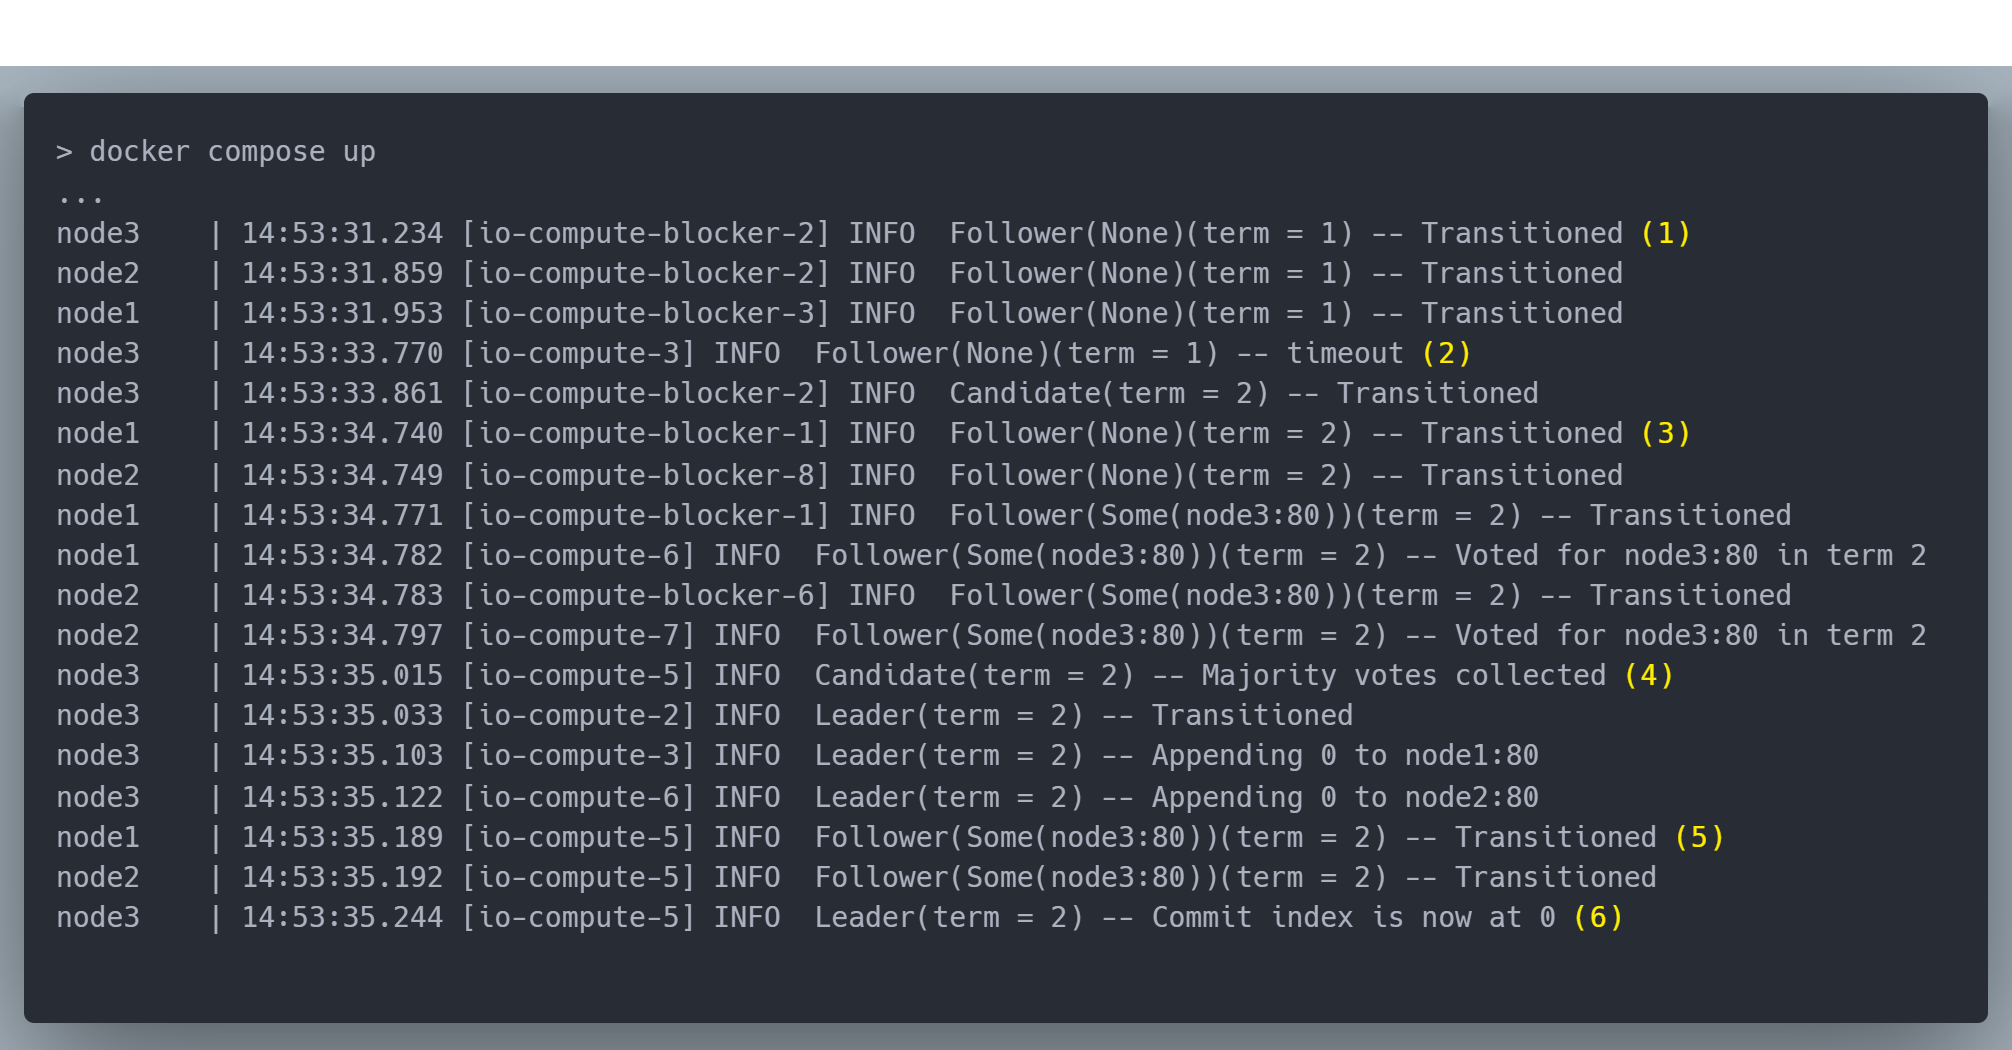
\includegraphics[width=500pt]{images/scenario_1.png}
\caption{Cluster output for the first scenario.}
\label{fig:scenario-1}
\end{figure}

\subsubsection{Result}

In Figure \ref{fig:scenario-1}, the following events are marked:
\begin{enumerate}
    \item After the initial startup, all three servers become followers for the first term.
    \item Since there is no leader in the cluster to send heartbeats, Server 3 becomes a candidate for the second term after an election timeout goes by and starts requesting votes from Server 1 and Server 2.
    \item Server 1 and Server 2 receive the vote requests, transition to followers in the second term, and vote for Server 3.
    \item Having collected votes from the majority, Server 3 transitions to a leader and informs its followers by sending an empty append request, at index 0.
    \item The followers respond to the append requests, recognizing Server 3 as the leader.
    \item Since the leader successfully replicated the entry at index 0, it is marked as committed, and the replicated state machine is ready for further input. The cluster remains stable thereafter, as the leader maintains its authority by sending heartbeat requests in the background.
\end{enumerate}

\subsubsection{Commentary}

Note that the entry at index 0 is virtual; it is not an actual entry in the log. It matches with the position in the follower's log right before the first entry, and the leader replicates it when its own log is empty.

\subsection{Recovery on Single Follower's Crash}

This scenario showcases how a cluster handles a follower's crash and recovery, with no requests being issued in between.

\subsubsection{Initial State}

The replicated log is empty and the cluster is stable with Server 1 as the leader, as shown under Marker 1 in Figure \ref{fig:scenario-2-cluster}.

\subsubsection{Input}

Two commands are executed via the terminal: \lstinline|docker stop node3|, which simulates a crash by stopping the container running Server 3, and \lstinline|docker start node3|, which simulates recovery by starting it up again. These are shown in Figure \ref{fig:scenario-2-commands}. Note that there is a delay of several seconds added between the execution of the two commands.

\begin{figure}[!ht]
\centering
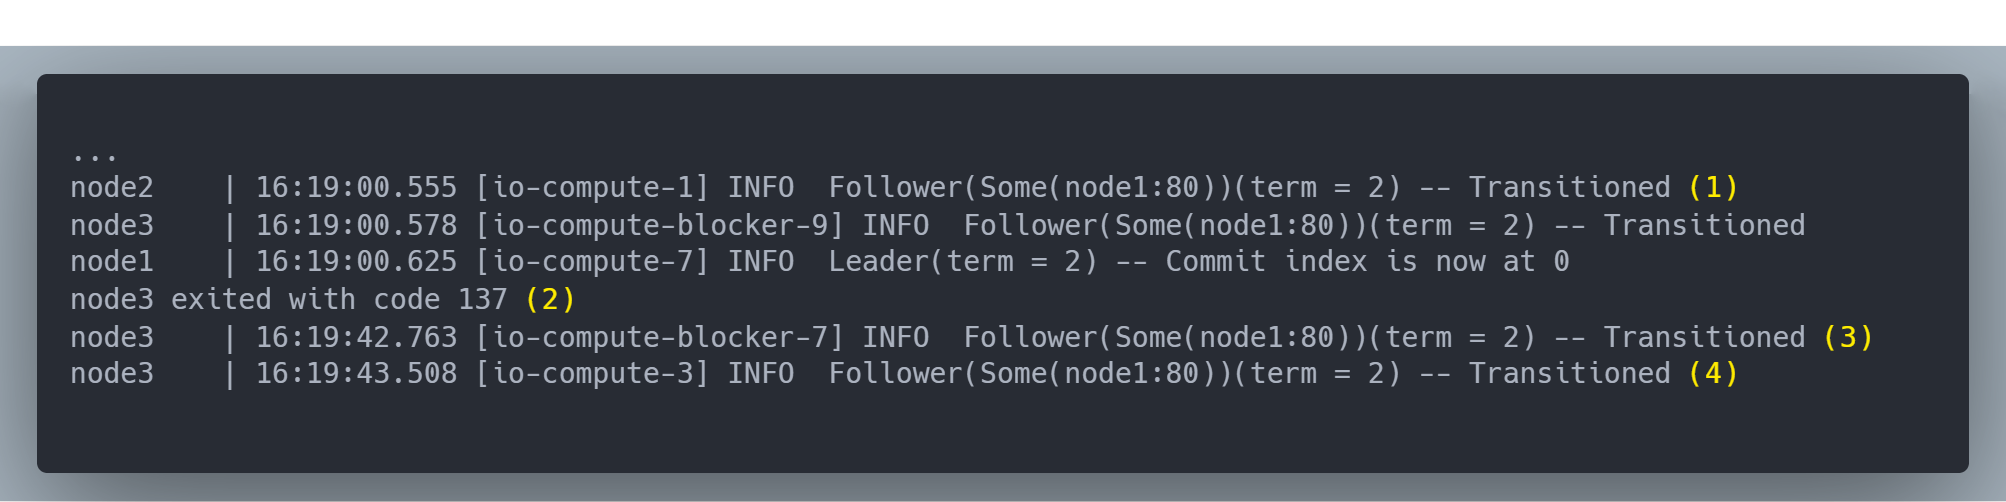
\includegraphics[width=500pt]{images/scenario_2_cluster.png}
\caption{Cluster output for the second scenario.}
\label{fig:scenario-2-cluster}

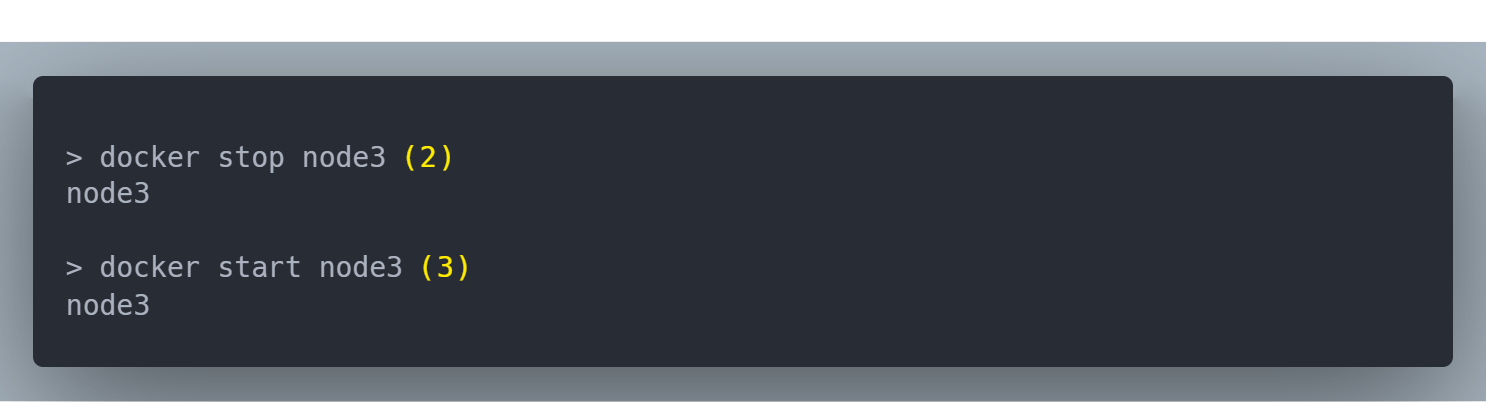
\includegraphics[width=500pt]{images/scenario_2_commands.png}
\caption{Input commands for the second scenario.}
\label{fig:scenario-2-commands}
\end{figure}

\subsubsection{Result}

In Figures \ref{fig:scenario-2-cluster} and \ref{fig:scenario-2-commands}, the following events are marked:
\begin{enumerate}
    \item The cluster is stable before any command is issued, with Server 1 being the leader and Servers 2 and 3 being followers.
    \item Server 3 is stopped via an external command.
    \item After several seconds, Server 3 is started up again.
    \item Server 3 learns again that Server 1 is the leader and remains as a follower. The cluster remains stable thereafter.
\end{enumerate}

\subsubsection{Commentary}

Note that the log message Marked as 4 is produced because the server learns of the leader's location in the cluster. This information is not persisted between server restarts, so it has to be re-learned. This is not clearly shown in the message, but it is proven by the server remaining as a follower and not transitioning to candidate after several election timeouts go by. 

\subsection{Recovery on Multiple Followers' Crash}

This scenario expands on the previous one by showing the cluster's behavior when all followers crash and later recover, with no requests being issued in between.

\subsubsection{Initial State}

The replicated log is empty and the cluster is stable with Server 3 as the leader, as shown under Marker 1 in Figure \ref{fig:scenario-3-cluster}.

\subsubsection{Input}

A crash is simulated in both follower servers by issuing \lstinline|docker stop| commands via the terminal. They are restarted after several seconds, by issuing \lstinline|docker start| commands. These are shown in Figure \ref{fig:scenario-3-commands}.

\begin{figure}[!ht]
\centering
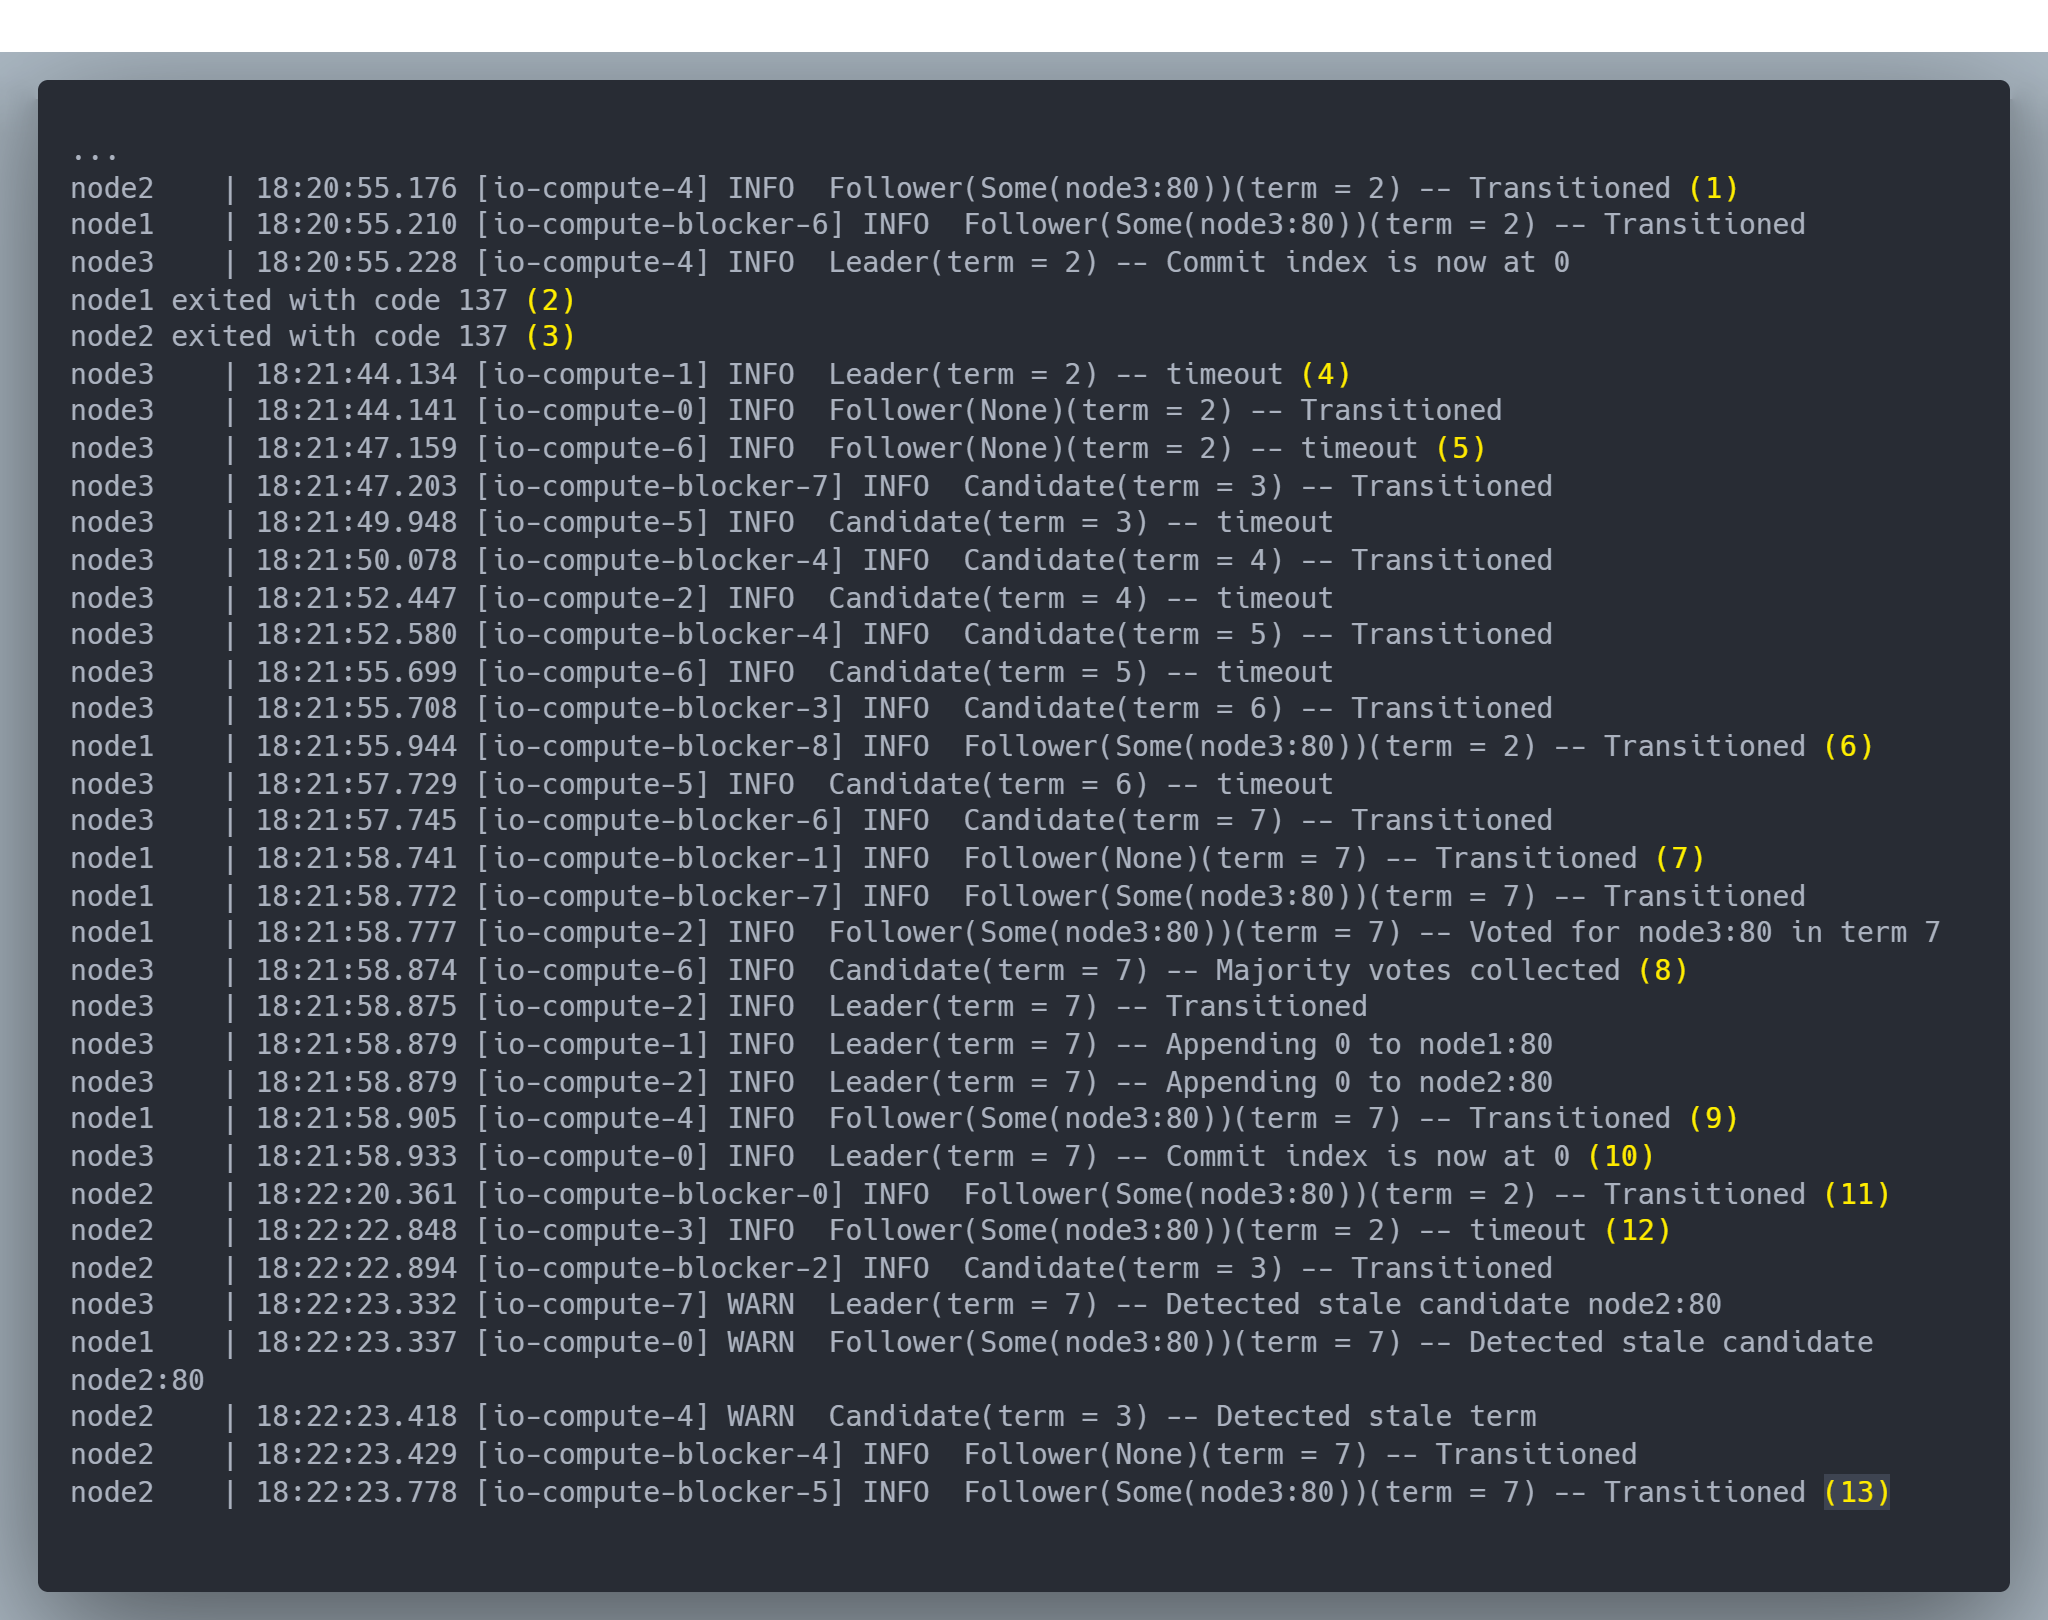
\includegraphics[width=500pt]{images/scenario_3_cluster.png}
\caption{Cluster output for the third scenario.}
\label{fig:scenario-3-cluster}
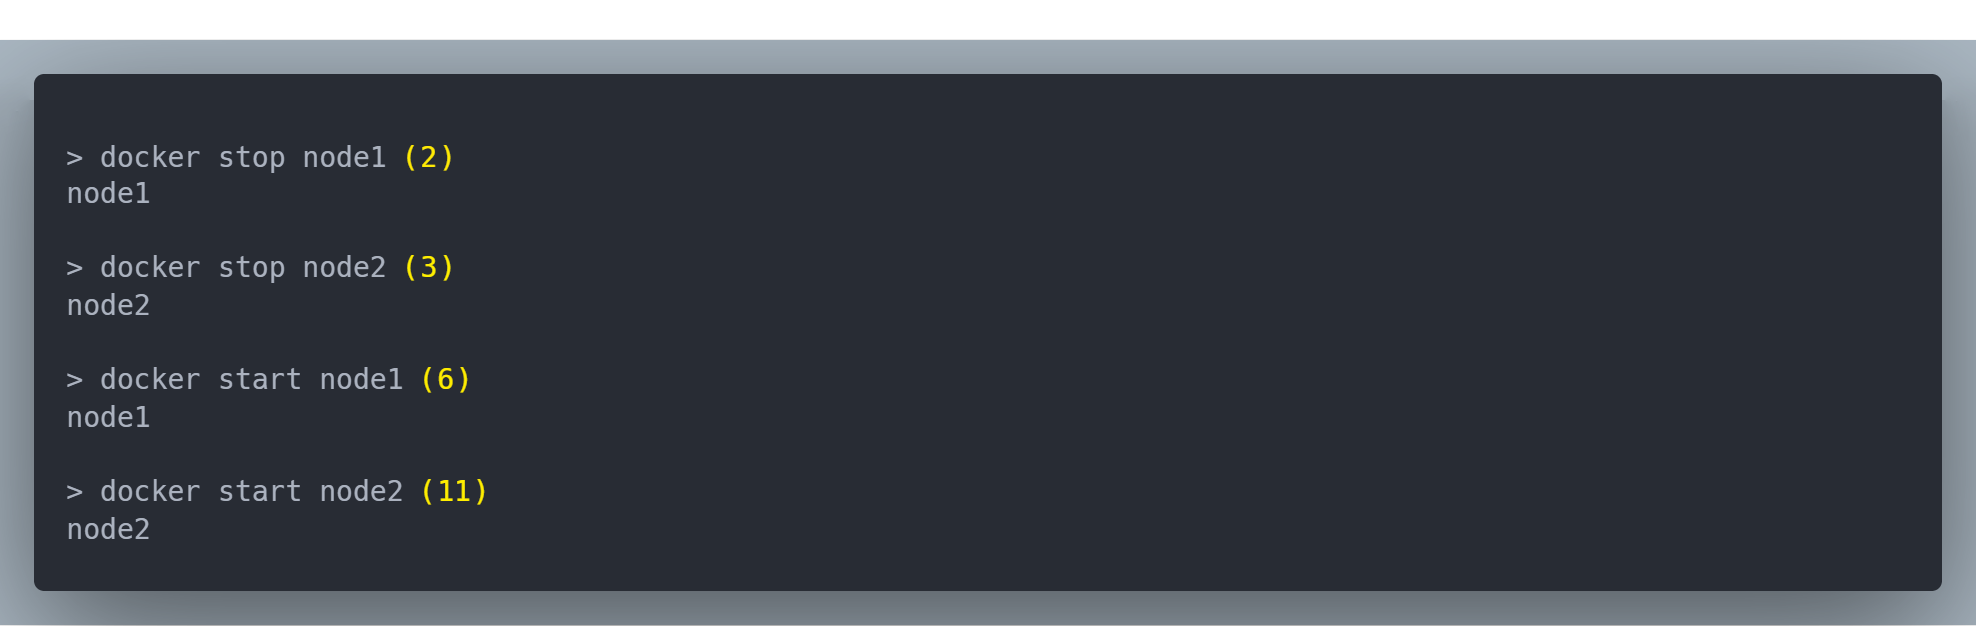
\includegraphics[width=500pt]{images/scenario_3_commands.png}
\caption{Input commands for the third scenario.}
\label{fig:scenario-3-commands}
\end{figure}

\subsubsection{Result}

In Figures \ref{fig:scenario-3-cluster} and \ref{fig:scenario-3-commands}, the following events are marked:
\begin{enumerate}
    \item The cluster is stable before any command is issued, with Server 3 being the leader and Servers 1 and 2 being followers.
    \item Server 1 is stopped via an external command.
    \item Server 2 is stopped via an external command.
    \item Server 3 is unable to reach a majority of the cluster. Since it cannot make progress, it reverts back to a follower for the current term.
    \item Server 3 transitions to a candidate for the next term after an election timeout and tries to gather votes. As no other servers are reachable, Server 3 goes through several election cycles with the term increasing each time, until a majority can be reached again.
    \item Server 1 is started up again. It has a stale term, as it has not observed any of the election cycles.
    \item Server 1 is reached by Server 3, which asks for a vote. Server 1 learns of the current term and votes for Server 3.
    \item Server 3 gathered a vote from Server 1, and since it has also implicitly voted for itself, it has collected a majority of votes and becomes the leader once more. Then, it attempts to replicate the virtual entry to the rest of the cluster, asserting its authority.
    \item Server 1 accepts the virtual entry which informs it that Server 3 is the leader for the current term.
    \item Server 3 has successfully replicated the virtual entry to the majority, so it is marked as committed.
    \item Server 2 is started up again and has a stale term.
    \item Server 2 happened to not observe the leader's heartbeats for an election timeout and transitioned to candidate. However, its vote requests are rejected by all other servers due to its stale term and it reverts to a follower. Additionally, the other servers inform Server 2 of the current term, so Server 2 adopts it.
    \item Server 2 finally receives heartbeats from the leader and recognizes it, remaining as a follower. The cluster then remains stable indefinitely.
\end{enumerate}

\subsubsection{Commentary}

These results show that in Raft clusters, and in distributed systems more broadly, there are hiccups during the consensus process that may cause a temporary divergence. However, Raft, and all successful consensus systems, guarantee that the servers will eventually reach a correct state.\\

In particular, events 11 and 12 show that Server 2 mistakenly became a candidate, which could be catastrophic in a naively implemented system. The candidate could gather votes and erroneously modify the replicated state machine, beginning at a stale view of the log. Raft guards against this type of error through its use of terms and its restrictions in the leader election and log replication processes, described in Chapter 2. As a result, stale servers cannot modify the replicated state machine, and the cluster will eventually be made consistent.

\subsection{Recovery on Leader's Crash}

This scenario showcases the cluster's recovery after the leader crashes. Additionally, it shows how a server that crashed while being the leader can later rejoin the cluster.

\subsubsection{Initial State}

The replicated log is empty and the cluster is stable with Server 1 as the leader, as shown under Marker
1 in Figure \ref{fig:scenario-4-cluster}.

\subsubsection{Input}

The leader is stopped via the terminal by issuing a \lstinline|docker stop| command. It is restarted after several seconds by issuing a \lstinline|docker start| command. These are shown in Figure \ref{fig:scenario-4-commands}.

\begin{figure}[!ht]
\centering
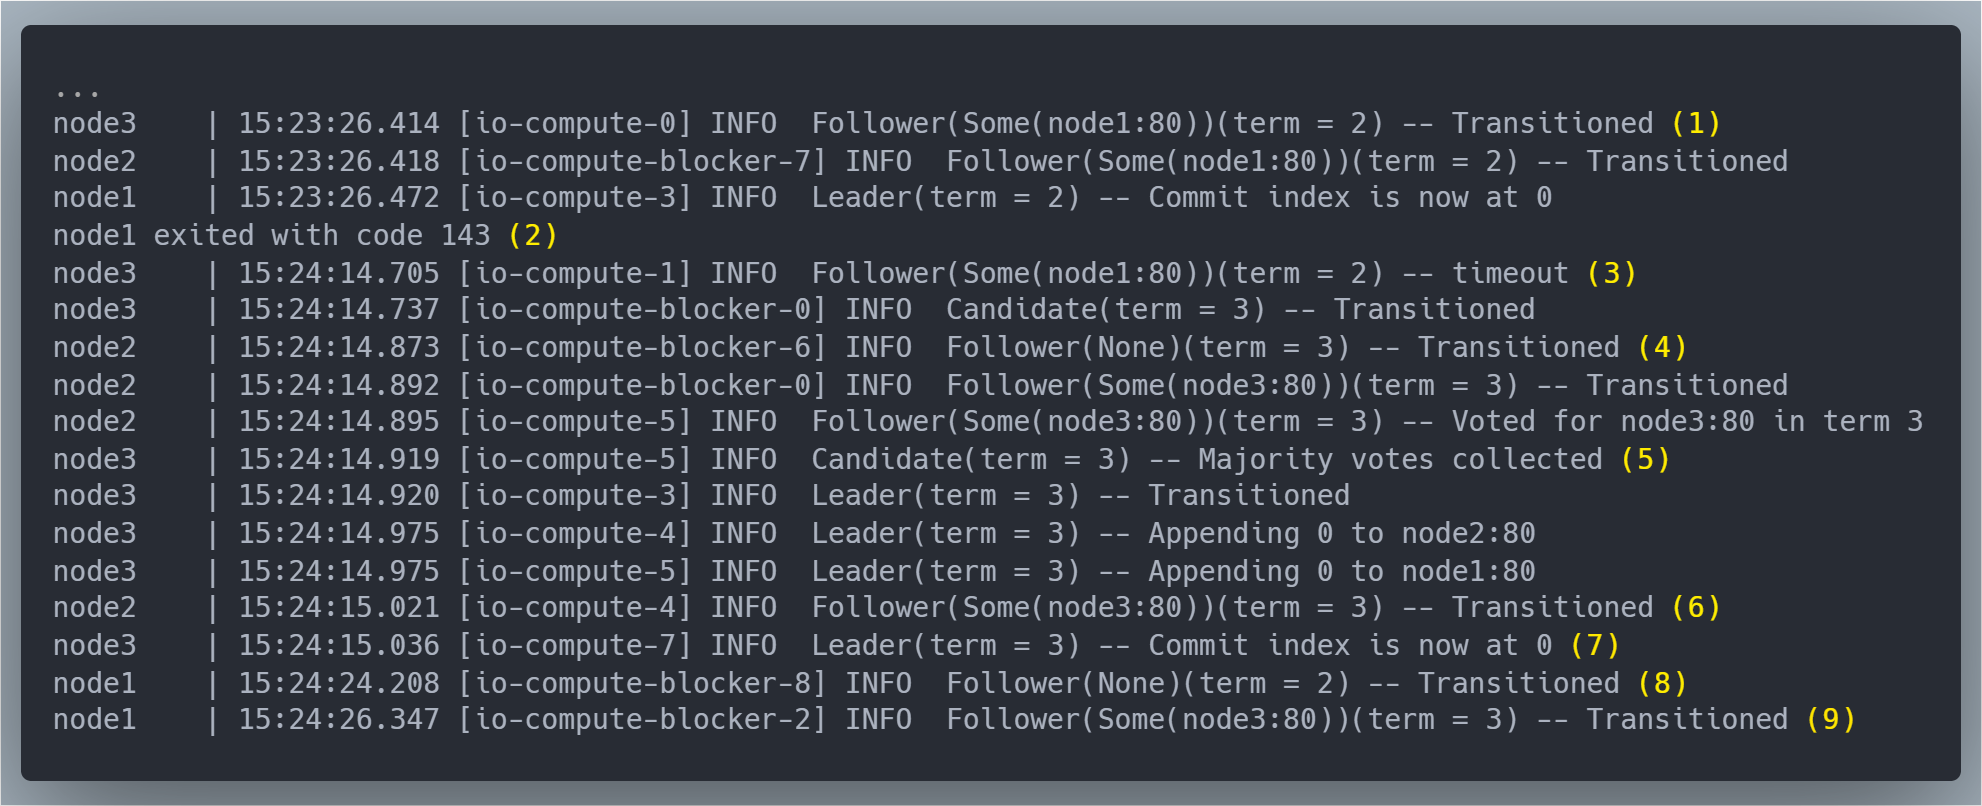
\includegraphics[width=500pt]{images/scenario_4_cluster.png}
\caption{Cluster output for the fourth scenario.}
\label{fig:scenario-4-cluster}
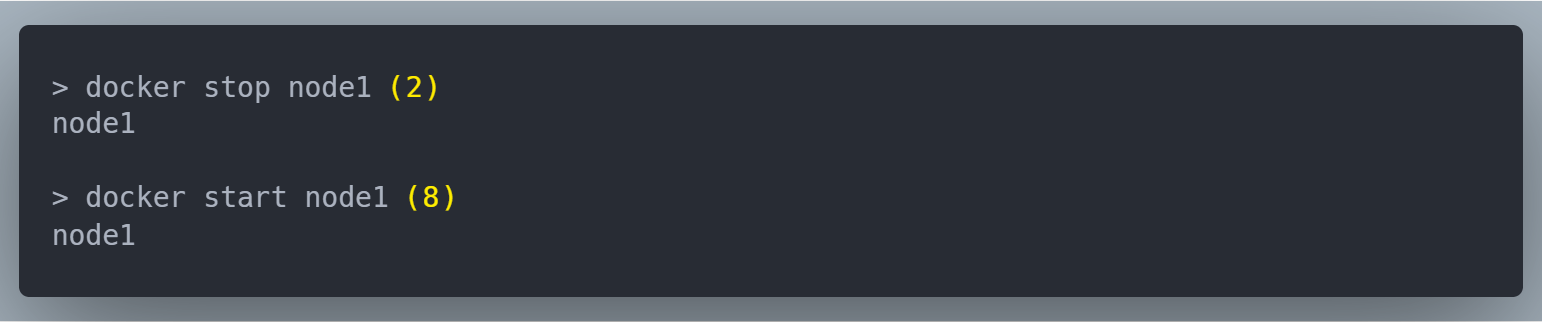
\includegraphics[width=500pt]{images/scenario_4_commands.png}
\caption{Input commands for the fourth scenario.}
\label{fig:scenario-4-commands}
\end{figure}

\subsubsection{Result}

In Figures \ref{fig:scenario-4-cluster} and \ref{fig:scenario-4-commands}, the following events are marked:
\begin{enumerate}
    \item The cluster is stable before any command is issued, with Server 1 being the leader and Servers 2 and 3 being followers.
    \item Server 1 is stopped via an external command.
    \item Server 3 detects that there is no viable leader, as it did not receive heartbeats for an election timeout. It then transitions to a candidate for the next term and requests that the rest of the cluster votes for it.
    \item Server 2 receives the vote request, learns the new term, and votes for Server 3.
    \item Server 3 has gathered votes from the majority of the cluster, as it has also implicitly voted for itself. It then transitions to a leader for the term, and it appends the virtual entry to the rest of the cluster, as its log is still empty.
    \item Server 2 accepts the append from Server 3, recognizing it as the leader.
    \item Server 3 successfully committed the virtual entry, as it is replicated to the majority of the cluster, including itself.
    \item Server 1 is started up again via an external command and joins the cluster as a follower. Its term is stale, since it did not observe any of the previous transitions.
    \item Server 1 receives a heartbeat from Server 3 and recognizes it as the leader. The cluster remains stable thereafter.
\end{enumerate}

\subsubsection{Commentary}

This scenario shows one of the fundamental requirements for a successful leader-based consensus system; progress continues even when the current leader fails by quickly and safely electing a new one.

\subsection{Recovery after Complete Cluster Termination}

This scenario showcases the cluster's ability to progress after completely failing and becoming operational again.

\subsubsection{Initial State}

The replicated log is empty and the cluster is stable with Server 2 as the leader, as shown under Marker 1 in Figure \ref{fig:scenario-5-cluster}.

\subsubsection{Input}

The entire cluster is completely shut down by issuing the \lstinline|docker compose down| command. After several seconds, the cluster is restarted by issuing the \lstinline|docker compose up -d| command. These are shown in Figure \ref{fig:scenario-5-commands}.

\begin{figure}[!ht]
\centering
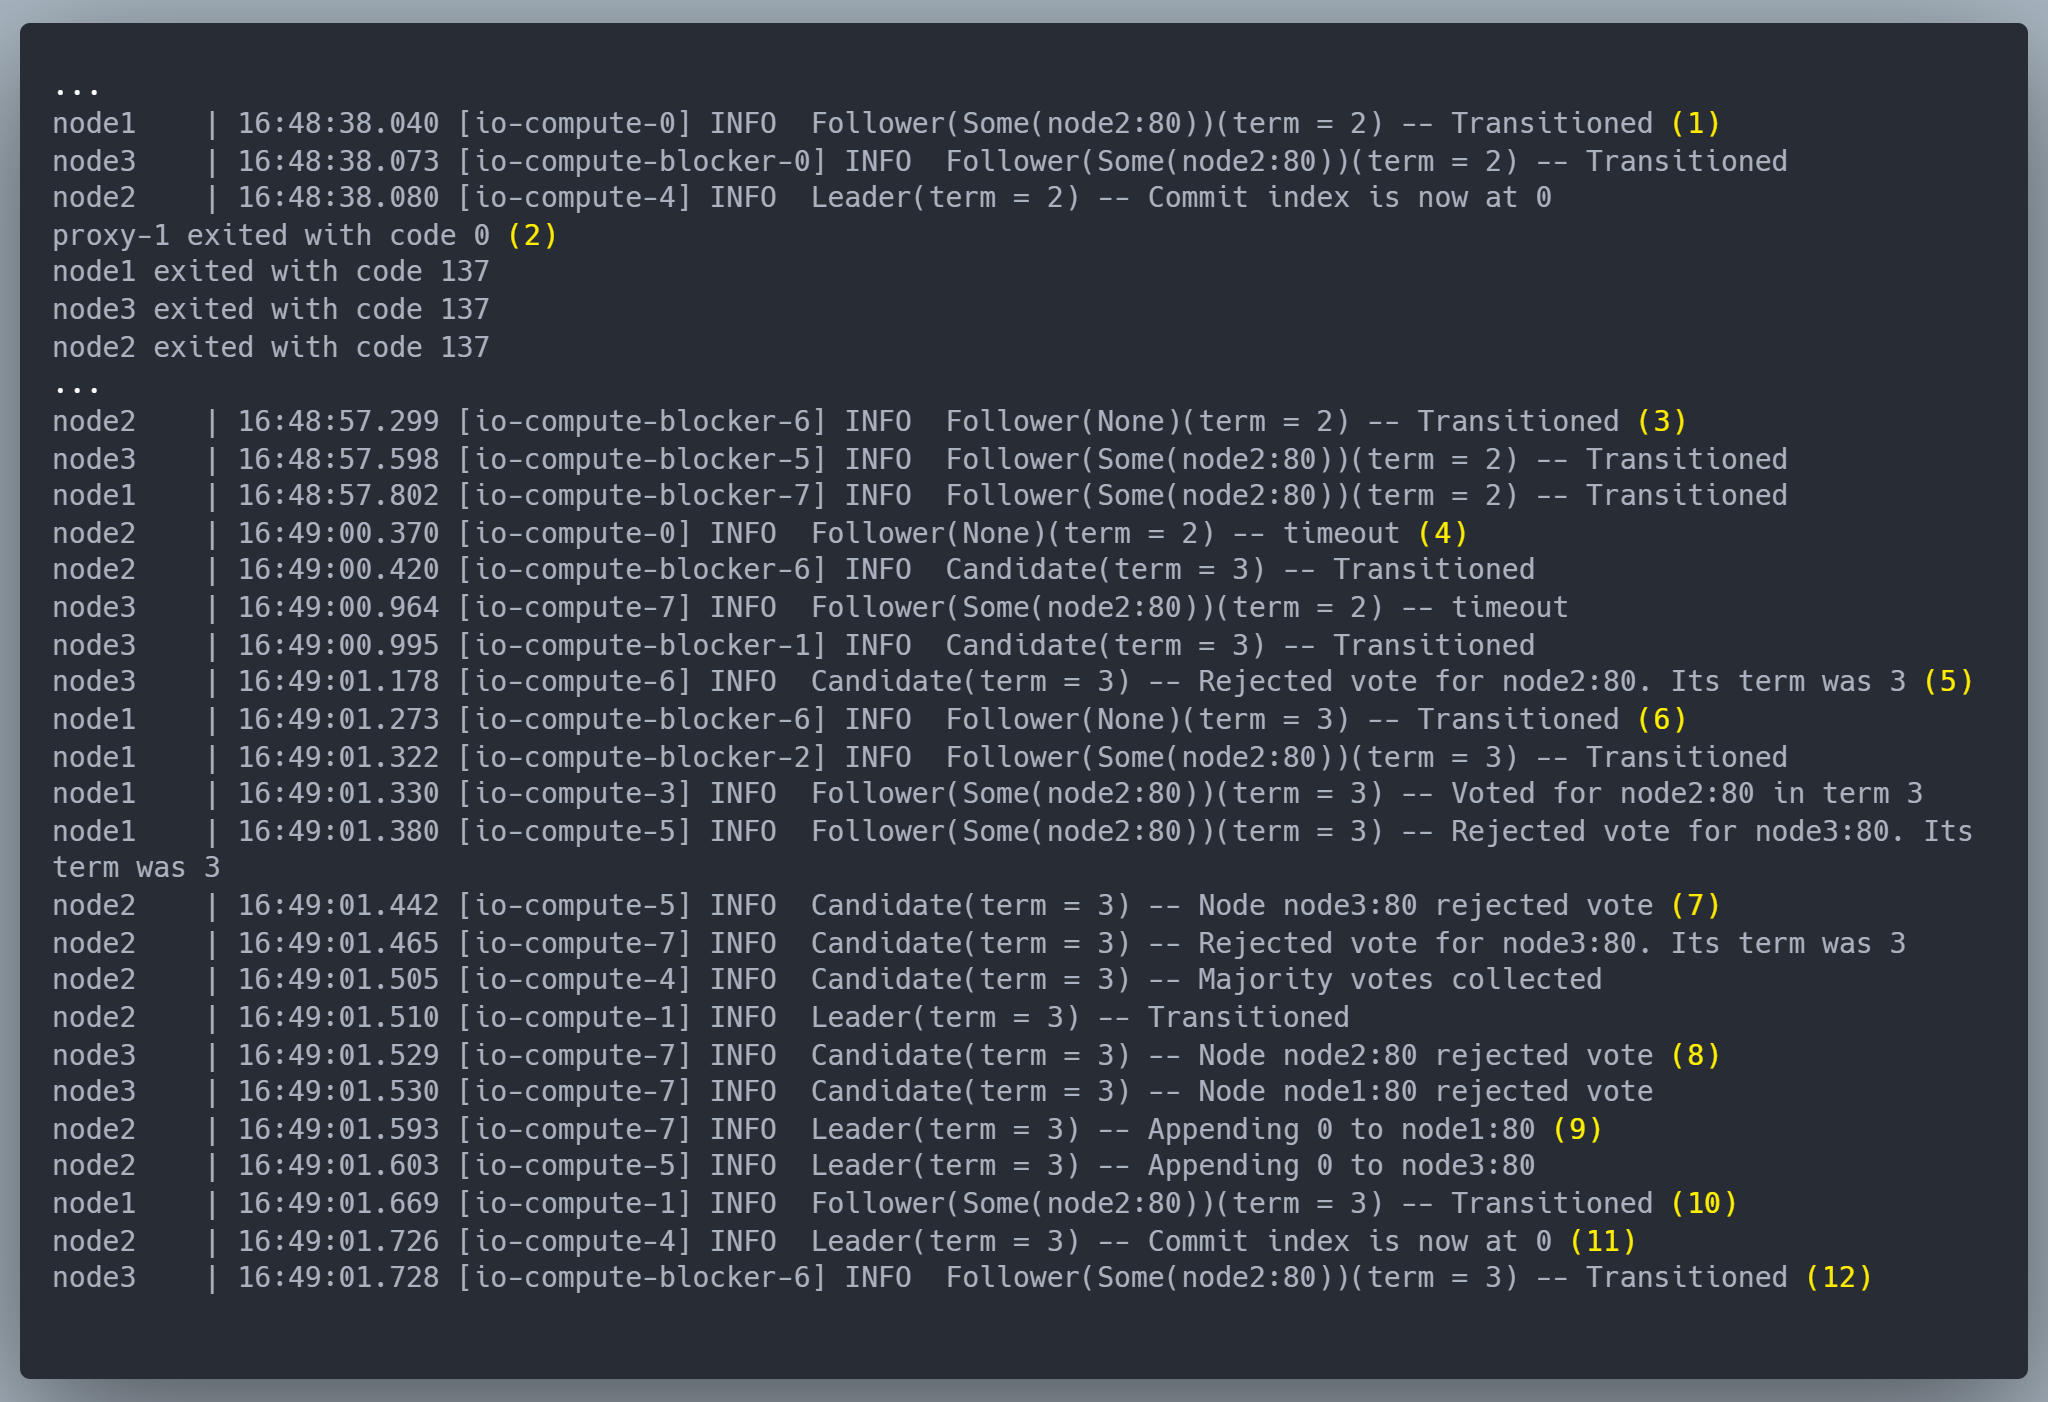
\includegraphics[width=500pt]{images/scenario_5_cluster.png}
\caption{Cluster output for the fifth scenario.}
\label{fig:scenario-5-cluster}
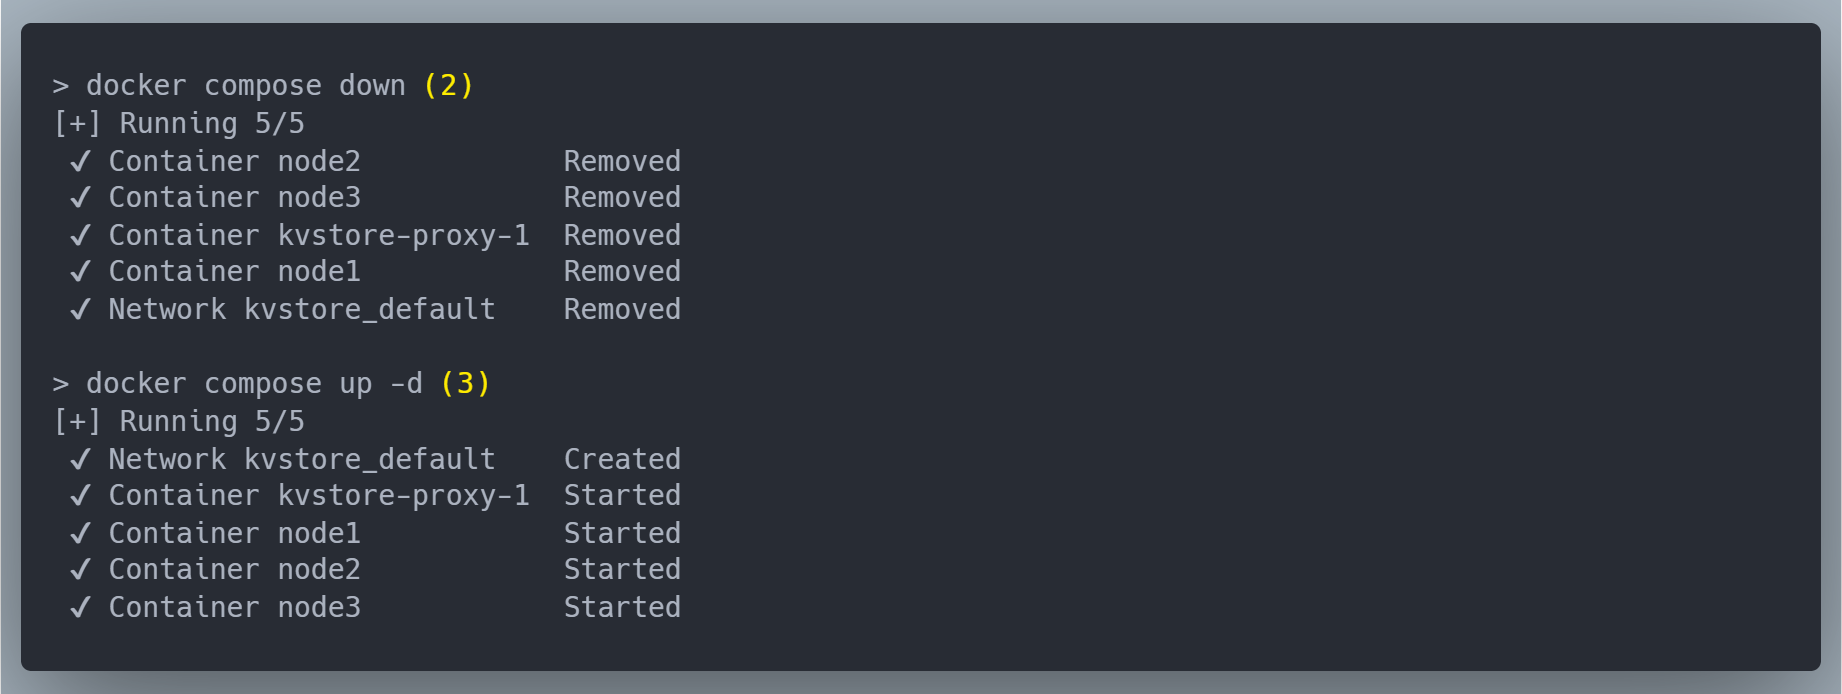
\includegraphics[width=500pt]{images/scenario_5_commands.png}
\caption{Input commands for the fifth scenario.}
\label{fig:scenario-5-commands}
\end{figure}

\subsubsection{Result}

In Figures \ref{fig:scenario-5-cluster} and \ref{fig:scenario-5-commands}, the following events are marked:
\begin{enumerate}
    \item The cluster is stable before any command is issued, with Server 2 being the leader and Servers 1 and 3 being followers. The Servers have reached the second term, since an election cycle happened during startup.
    \item The cluster is shut down via an external command.
    \item After several seconds, the cluster is restarted via an external command. All servers join as followers with the term they knew of before they were shut down.
    \item Both Server 2 and Server 3 experience election timeouts in quick succession. They transition to candidates for the next term and attempt to gather votes.
    \item Server 3 rejects to vote for Server 2, as it has already implicitly voted for itself.
    \item Server 1 receives the vote request from Server 2 before the request from Server 3. It then grants the vote to Server 2 and rejects Server 3.
    \item Server 2 learns that Server 3 rejected its vote request, but Server 1 granted it. Since Server 2 has also implicitly voted for itself, it has received votes by the majority, and it transitions to a leader for the term. Server 2 also rejects the vote request it received from Server 3.
    \item Server 3 learns of the other servers' rejections. Since it has not received a majority of votes, it remains as a candidate.
    \item Server 2, acting as a leader, starts appending the virtual entry to other servers, informing them of its victory.
    \item Server 1 responds to the append from Server 2, recognizing it as the leader.
    \item After Server 1 responds, the leader has successfully committed the virtual entry.
    \item Server 3 also responds to the append from Server 2, recognizing it as the leader and transitioning to a follower.
\end{enumerate}

\subsubsection{Commentary}

These results show how the persistence layer is used to preserve any required information through complete system crashes or restarts. It also showcases how the leader election process, as defined by Raft, succeeds, even when an unfortunate timing of the election timeouts leads to multiple candidates for a term.

\subsection{Simple Get and Put Commands} \label{simple-get-put-scenario} \label{L-flag}

This scenario showcases the key-value store in action by issuing simple read and write requests.

\subsubsection{Initial State}

The replicated log is empty and the cluster is stable with Server 1 as the leader, as shown under Marker 1 in Figure \ref{fig:scenario-6-cluster}.

\subsubsection{Input}

As shown in Figure \ref{fig:scenario-6-commands}, the \lstinline|curl| command is used to send HTTP requests to the store. Additionally, the \lstinline|uuidgen| command is used to generate unique command identifiers, which are required for enforcing linearizable semantics, as detailed in Section \ref{linearizable-semantics}.\\

All commands are issued with the \lstinline|-L| flag, instructing \lstinline|curl| to follow redirects. This is necessary as requests are issued against the proxy without specifying the target server. If the server to which the proxy initially routes the request is not the leader, it returns a redirection response. Curl then follows this redirection response and addresses the leader directly.\\

Note that it is possible to find out the location of the current leader once and then address it directly without further redirections. However, this was avoided to keep the demonstration simple.

\begin{figure}[!ht]
\centering
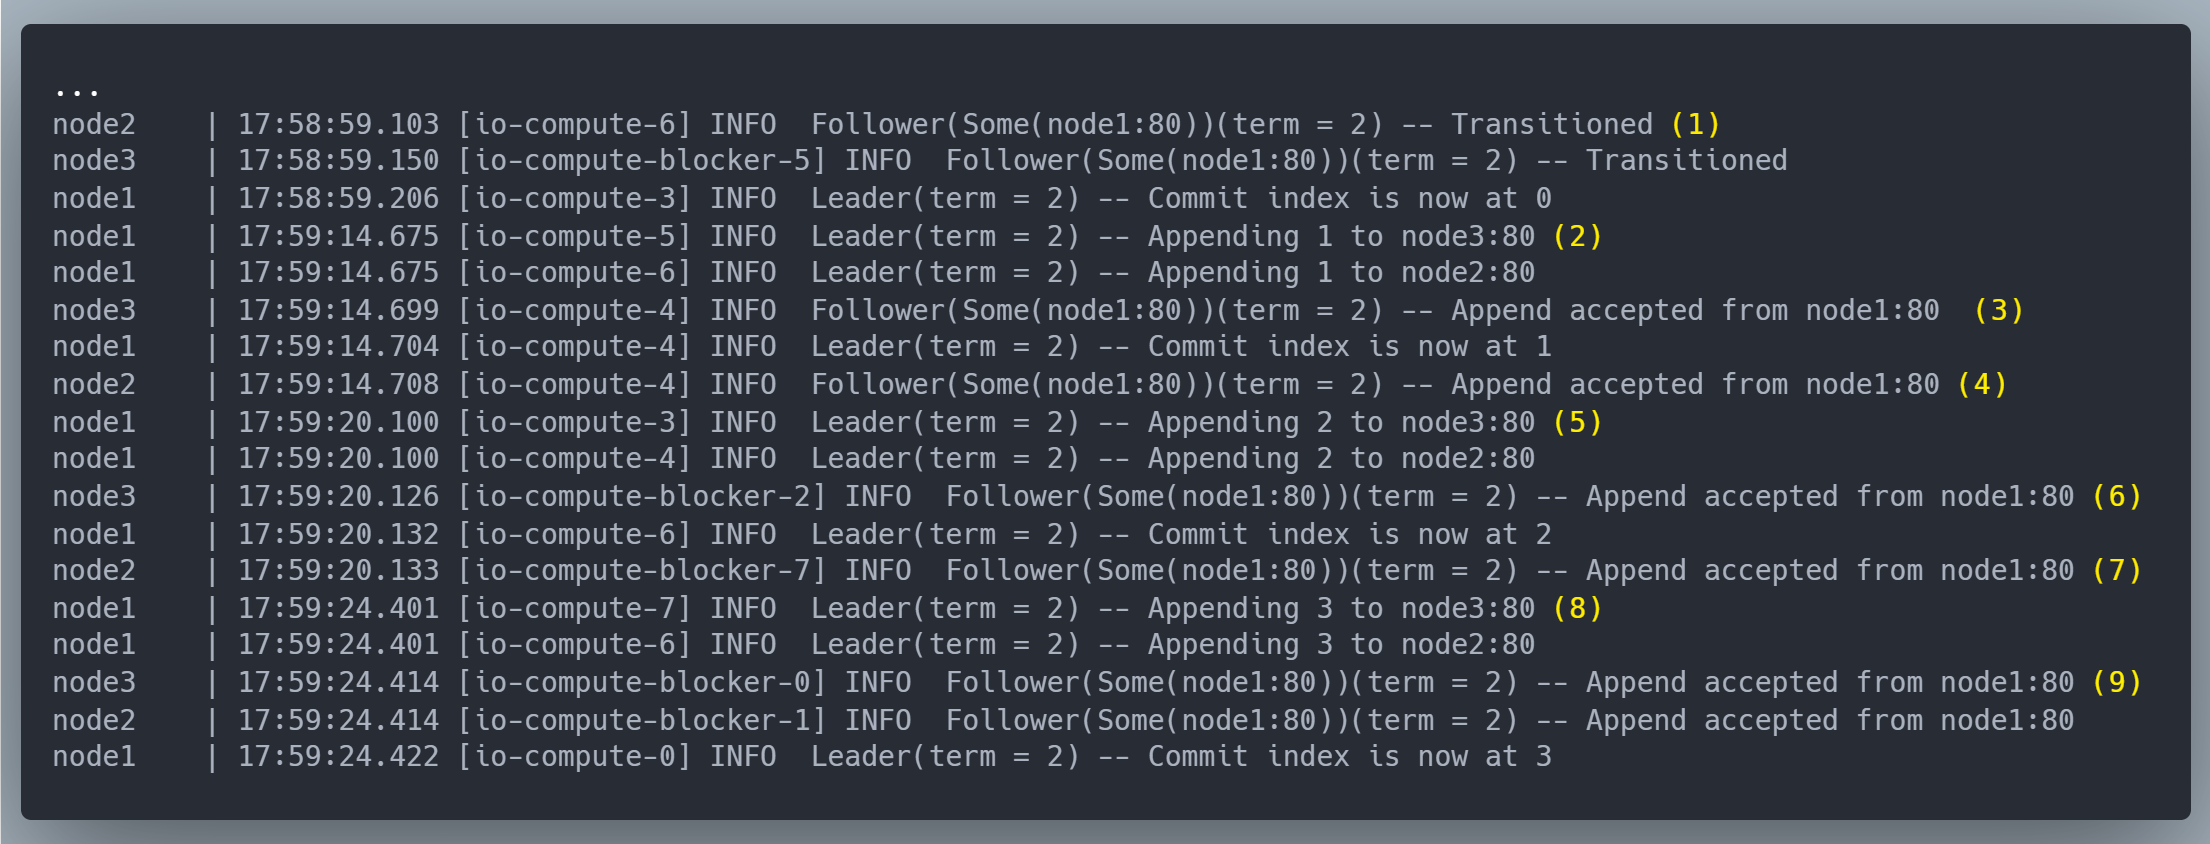
\includegraphics[width=500pt]{images/scenario_6_cluster.png}
\caption{Cluster output for the sixth scenario.}
\label{fig:scenario-6-cluster}
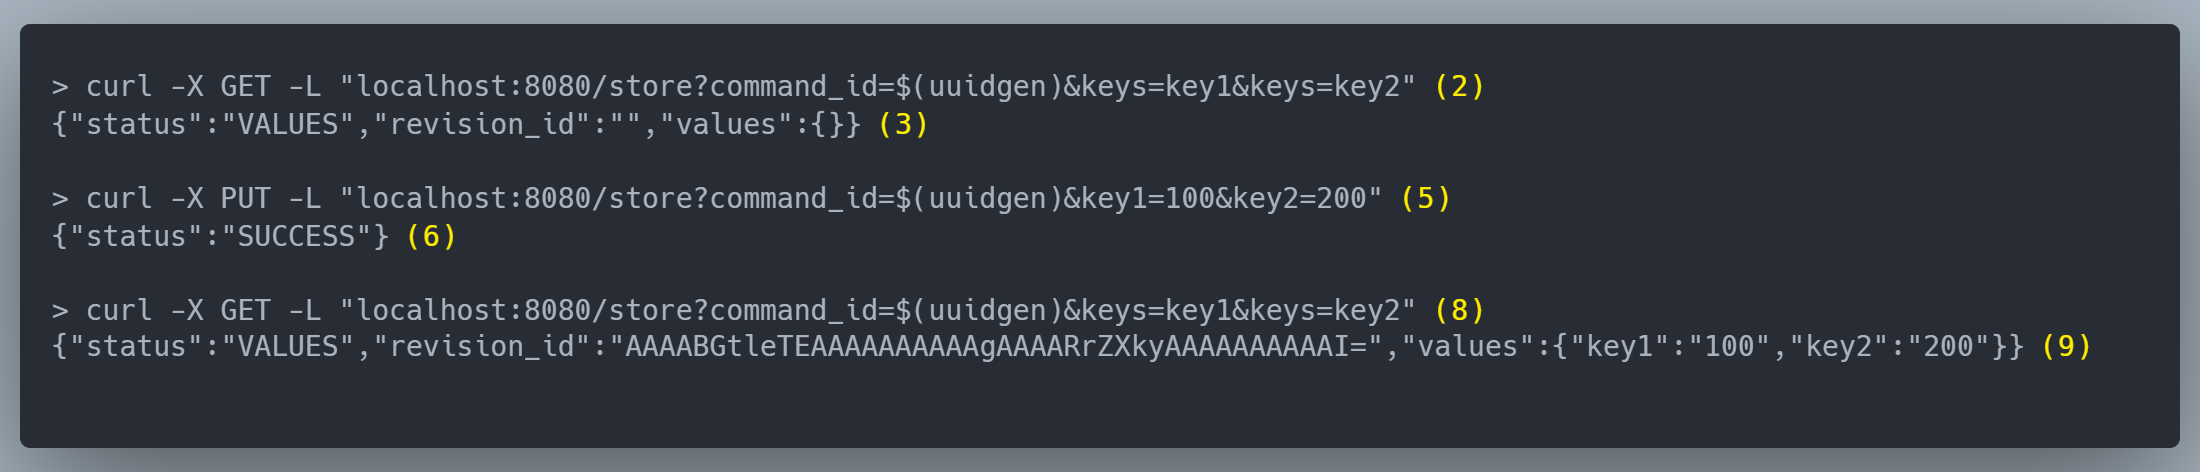
\includegraphics[width=500pt]{images/scenario_6_commands.png}
\caption{Input commands for the sixth scenario.}
\label{fig:scenario-6-commands}
\end{figure}

\subsubsection{Result}
In Figures \ref{fig:scenario-6-cluster} and \ref{fig:scenario-6-commands}, the following events are marked:
\begin{enumerate}
    \item The cluster is stable before any command is issued, with Server 1 being the leader and Servers 2 and 3 being followers.
    \item A client requests to view the values for keys \lstinline|key1| and \lstinline|key2|. As detailed in Section \ref{linearizable-semantics}, read requests are committed to the replicated log like any other command, so the replication process begins; Server 1, acting as the leader, sends append requests to its followers.
    \item Server 3 accepts the append first, inserting the command to its internal log, and responding to the leader. After this follower's response, the leader has successfully replicated the command to the majority of the cluster, including itself, and it increments the commit index. At that point, the client receives a response to its request, which contains no key-value pairs, since the store is empty.
    \item Server 2 also accepts the leader's append request.
    \item A client requests to insert the key-value pairs \lstinline|(key1,100)| and \lstinline|(key2,200)|. The replication process for the command begins with the leader sending append requests to its followers.
    \item Server 3 accepts the append first, inserting the command to its internal log, and responding to the leader. After this follower's response, the command is deemed committed, and the commit index is incremented. At that point, the client receives a response to its request, which shows that the insertion was successful.
    \item Server 2 also accepts the leader's append request.
    \item A client requests to view the values for keys \lstinline|key1| and \lstinline|key2|. The replication process for the command begins with the leader sending append requests to its followers.
    \item Both followers accept the append in quick succession, inserting the command to their internal logs, and responding to the leader. After the followers' responses, the leader has successfully replicated the command to the cluster and it increments the commit index. At that point, the client receives a response to its request, showing the requested key-value pairs. Along with the pairs, a revision id is returned, which marks the returned keys' current state.
\end{enumerate}

\subsection{Concurrent Get and Put Commands}

This scenario shows the store's behavior when multiple clients attempt to modify it concurrently, without using the provided transaction mechanism. It should show that the store reaches consensus properly about the replicated log, but the resulting state of the store is not the expected one, clearly showing the need for transactions.

\subsubsection{Initial State}

The replicated log is empty and the cluster is stable with Server 3 as the leader, as shown under Marker 1 in Figure \ref{fig:scenario-7-cluster}.

\subsubsection{Input}

The script \lstinline{concurrent_read_writes} is used for performing reads and writes concurrently. It interacts with the key-value store via HTTP requests, similarly to the previous scenario. Its source code can be found in the GitHub repository \cite{stoufexis-raft}.\\

The script takes three positional parameters: a string instructing to use or not use transactions, the number of keys to modify, and the number of processes concurrently modifying each key. The script figures out exactly which keys it will read and write to by starting at \lstinline|key1| and incrementing it until it has reached the number in the second parameter.\\

In the command shown in Figure \ref{fig:scenario-7-commands}, transactions are turned off, the set of keys from \lstinline|key1| to \lstinline|key10| is picked, and 10 concurrent processes are assigned to each key. In total, 100 processes will be running concurrently, which the script calls "workers".\\

As soon as the command is issued, the script initializes all keys to a value of 1 via a \lstinline|PUT| request. Then, it starts all concurrent processes, with each one reading the key's current value using a \lstinline|GET| request, incrementing it by 1, and inserting the result using a \lstinline|PUT| request. In the end, it reads all keys again, returning their final values. The goal is for each key to reach a value of 11, since they are all incremented 10 times, once by each worker.

\begin{figure}[!ht]
\centering
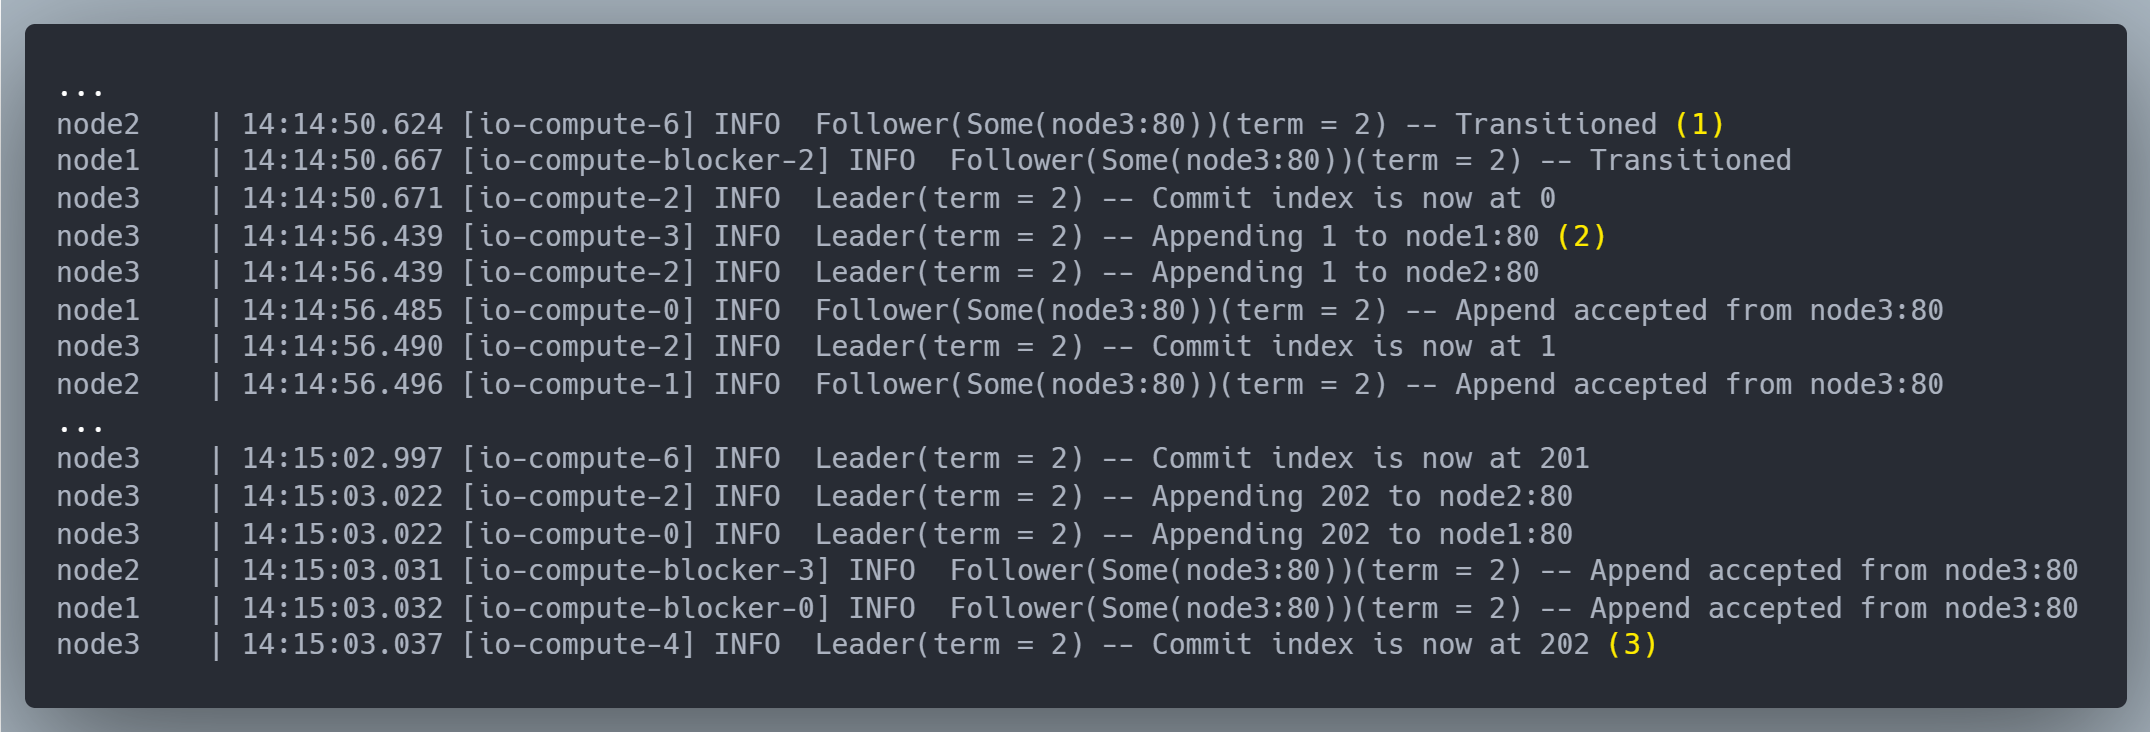
\includegraphics[width=500pt]{images/scenario_7_cluster.png}
\caption{Cluster output for the seventh scenario.}
\label{fig:scenario-7-cluster}
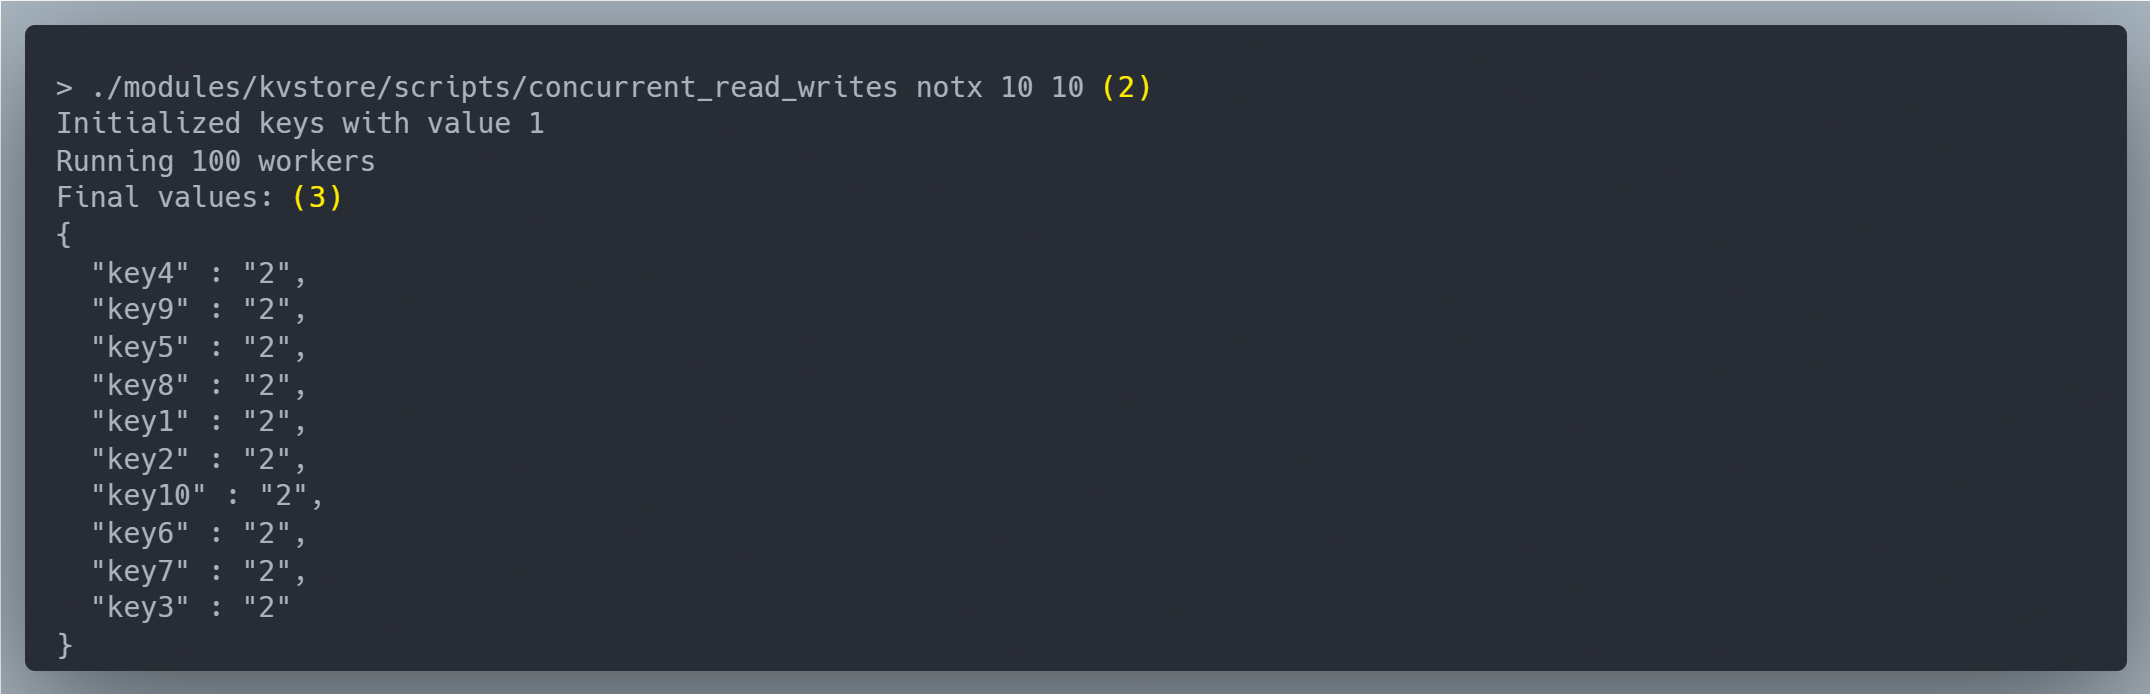
\includegraphics[width=500pt]{images/scenario_7_commands.png}
\caption{Input commands for the seventh scenario.}
\label{fig:scenario-7-commands}
\end{figure}

\subsubsection{Result}
In Figures \ref{fig:scenario-7-cluster} and \ref{fig:scenario-7-commands}, the following events are marked:
\begin{enumerate}
    \item The cluster is stable before any command is issued, with Server 3 being the leader and Servers 1 and 2 being followers.
    \item The script is run externally, which initializes the key-set and then starts up the concurrent workers.
    \item When all 202 commands have been processed, the script reads the keys' final values and returns them.
\end{enumerate}

\subsubsection{Commentary}
Several things are noteworthy in these results. First, in Figure \ref{fig:scenario-7-cluster}, it's shown that the commit index ends up at 202. This is correct, as there was one command issued for the initialization of the keys, 200 commands issued by the 10 concurrent processes, and one command issued for reading the final values. The concurrent processes issued 10 pairs of reads and writes for each key.\\

These results also prove that the Raft implementation is capable of handling concurrent requests from clients, since it reached consensus on the replicated log. However, in this case, the final values are not the desired ones. As transactions were turned off, each read and write pair did not get executed atomically, meaning that each worker ignored the other workers' modifications. In detail, this is what took place:
\begin{enumerate}
    \item All workers read the initial value of 1, before it is incremented.
    \item All workers calculate the incremented value as 2.
    \item Each worker updates the key's value to 2, not knowing that other modifications happened after the initial value was read.
\end{enumerate}

This should clearly demonstrate that a transaction mechanism is necessary to simultaneously support both concurrency and atomicity.

\subsection{Concurrent, Transactional Get and Put Commands} \label{transactions-scenario}
This scenario expands on the previous one by repeating the same actions, but this time using transactions. It should show that each read and write pair is retried until it is made atomically, leading to the expected final value.

\subsubsection{Initial State}

The replicated log is empty and the cluster is stable with Server 1 as the leader, as shown under Marker 1 in Figure \ref{fig:scenario-8-cluster}.

\subsubsection{Input}

As in the previous scenario, the script \lstinline{concurrent_read_writes} is used. However, as shown in Figure \ref{fig:scenario-8-commands}, this time it is instructed to use transactions. Transactions, as described in Section \ref{implementing-transactions}, ensure that each update is executed only if it is made atomically with the preceding read.\\

\begin{figure}[!ht]
\centering
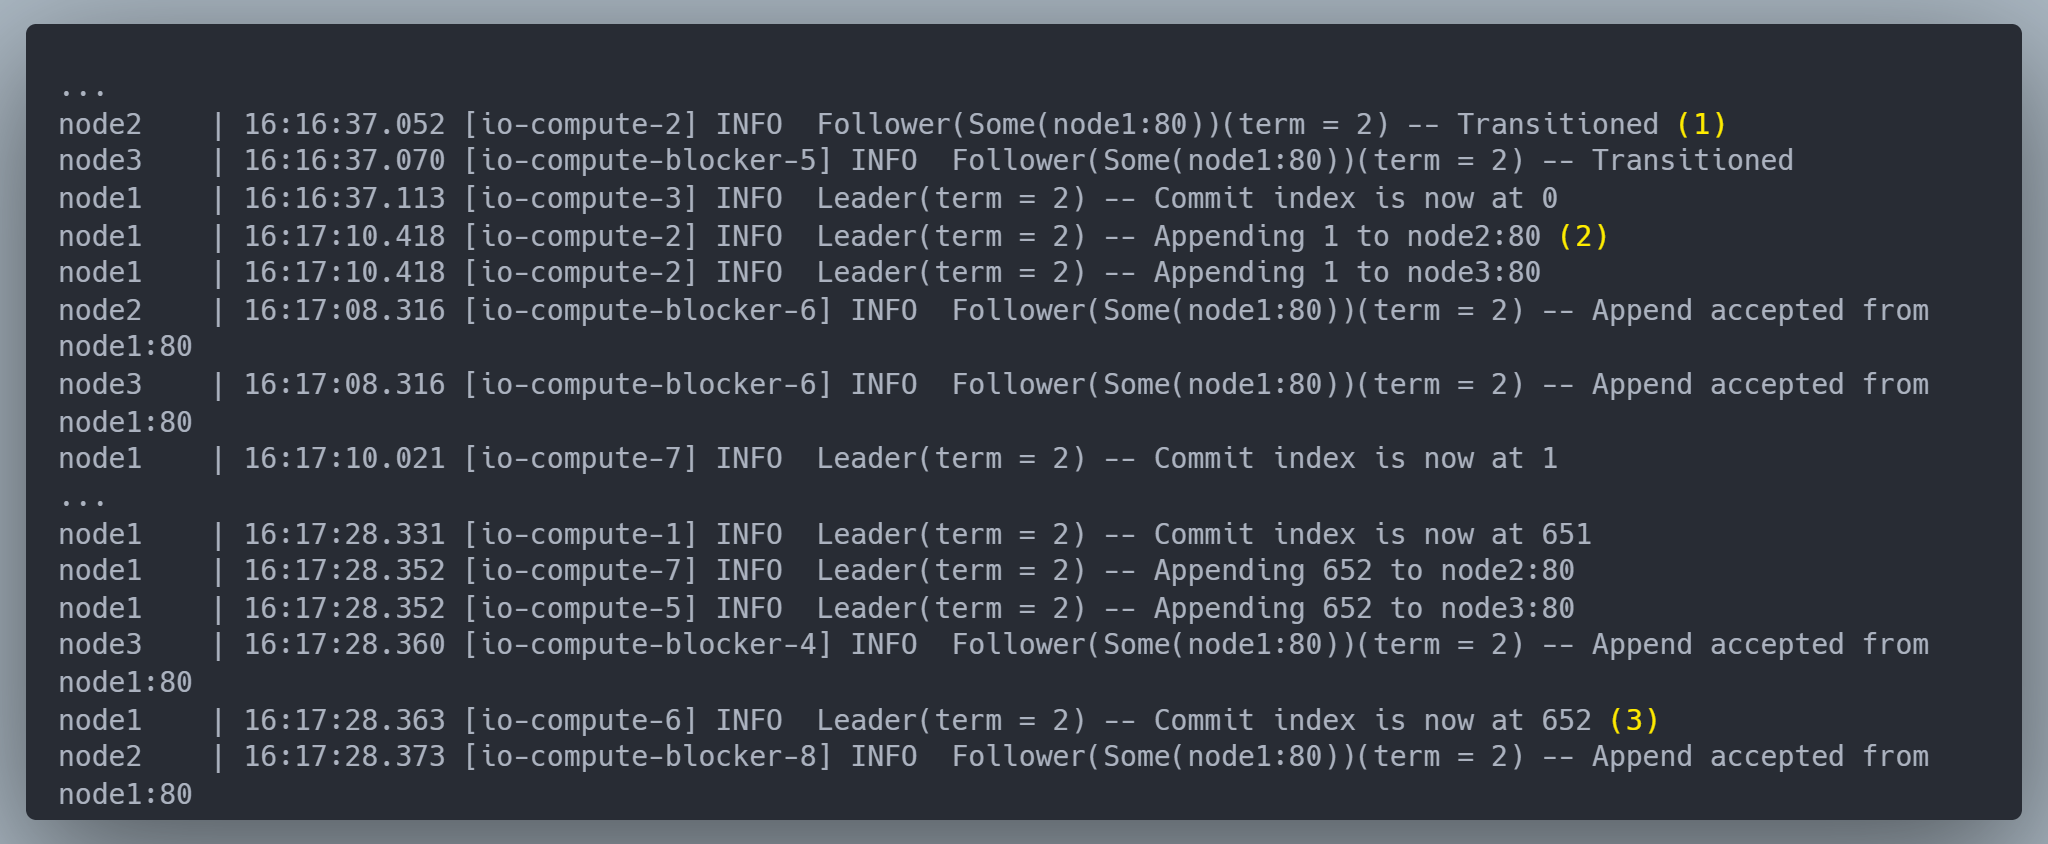
\includegraphics[width=500pt]{images/scenario_8_cluster.png}
\caption{Cluster output for the eighth scenario.}
\label{fig:scenario-8-cluster}
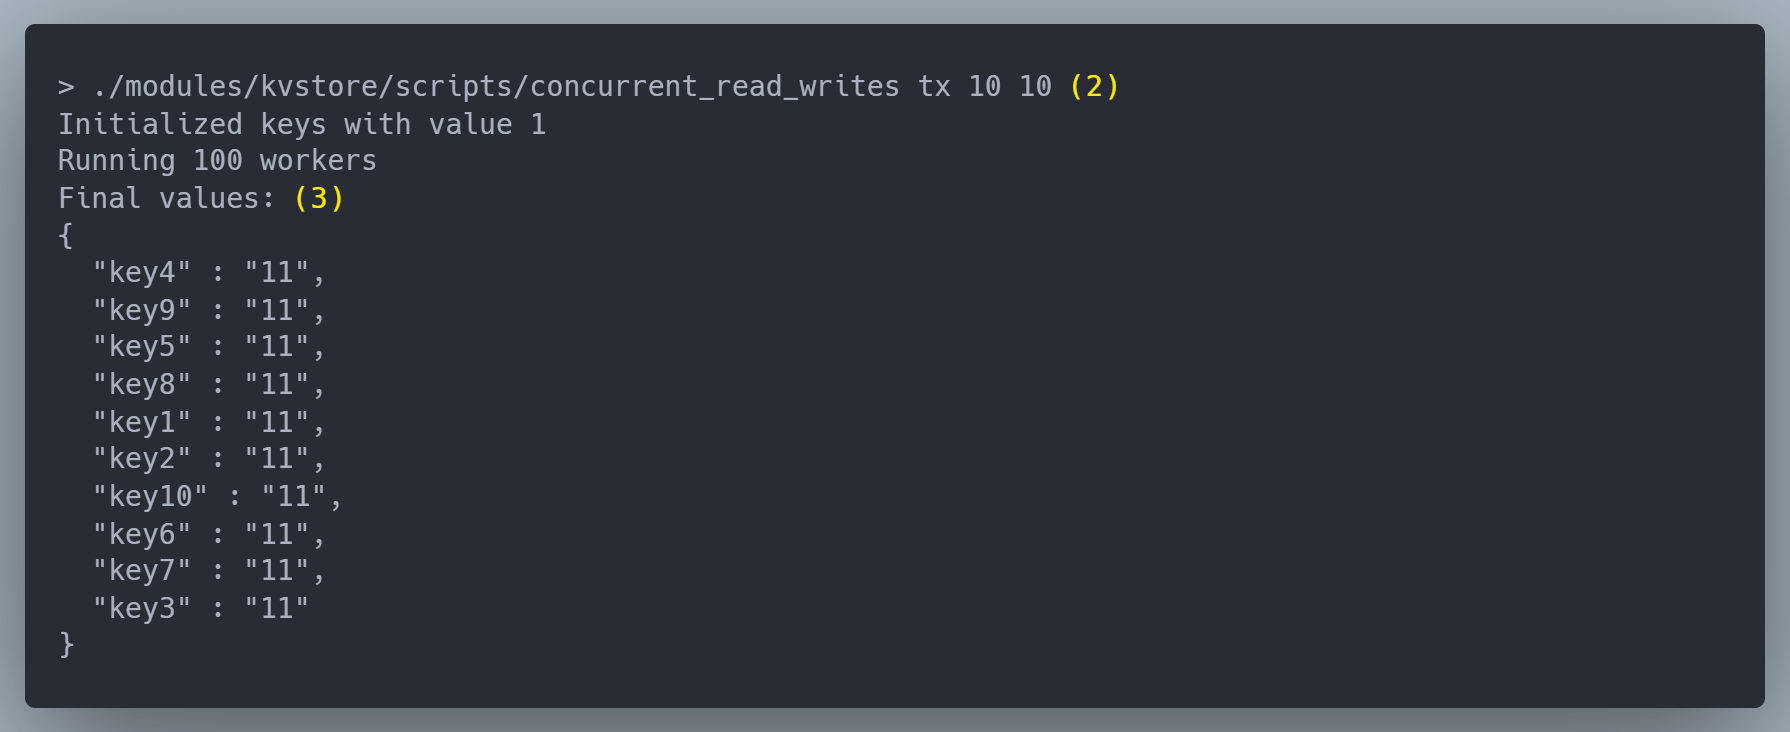
\includegraphics[width=500pt]{images/scenario_8_commands.png}
\caption{Input commands for the eighth scenario.}
\label{fig:scenario-8-commands}
\end{figure}

\subsubsection{Result}
In Figures \ref{fig:scenario-8-cluster} and \ref{fig:scenario-8-commands}, the following events are marked:
\begin{enumerate}
    \item The cluster is stable before any command is issued, with Server 1 being the leader and Servers 2 and 3 being followers.
    \item The script is run externally, which initializes the key-set and then starts up the concurrent workers.
    \item The script ends up generating 652 commands. At that point, the script terminates, showing the final values.
\end{enumerate}

\subsubsection{Commentary}

These results show that it is possible to achieve both concurrency and atomicity when using the implemented transaction mechanism, as all keys correctly reached the expected value of 11.\\

It is also shown that, due to the high contention between the concurrent workers, there were significantly more commands generated than the non-transactional example. With this setup, the theoretical maximum for commands is 652. This is calculated by first taking the commands that were required in the previous scenario, 202, which did not include any retries. Then, the maximum number of retry requests that would have to be sent on each iteration is added. For the first iteration, at worst 9 workers will have to retry for each of the 10 keys, issuing 90 requests. On the second iteration, at worst 8 workers would retry, issuing 80 requests, and so on, so fourth, resulting in the following expression:
\begin{equation}
202 + \sum_{n=1}^{9} ({100-10n}) = 652.
\end{equation}

The theoretical maximum was actually reached with this test setup, since it simulates the worst-case scenario; each iteration is timed so that the most workers possible will have to retry. However, in real-world cases, the number of needed commands would be greatly reduced, as requests would not be purposefully timed to conflict.

\subsection{Issuing Commands to the Cluster Between a Server's Crash and Recovery}

This scenario shows Raft's ability to catch up servers that missed commands due to crashes or other failures.

\subsubsection{Initial State}

The replicated log is empty and the cluster is stable with Server 2 as the leader, as shown under Marker 1 in Figure \ref{fig:scenario-9-cluster}.

\subsubsection{Input}

As shown in Figure \ref{fig:scenario-9-commands}, the \lstinline|docker stop| command is issued to simulate a failure on the leader server. Then, similarly to Scenario \ref{simple-get-put-scenario}, a series of requests is made to the store using \lstinline|curl|. In this case, three \lstinline|PUT| requests are made, each time inserting a unique key-value pair. Finally, the stopped server is restarted.

\begin{figure}[!ht]
\centering
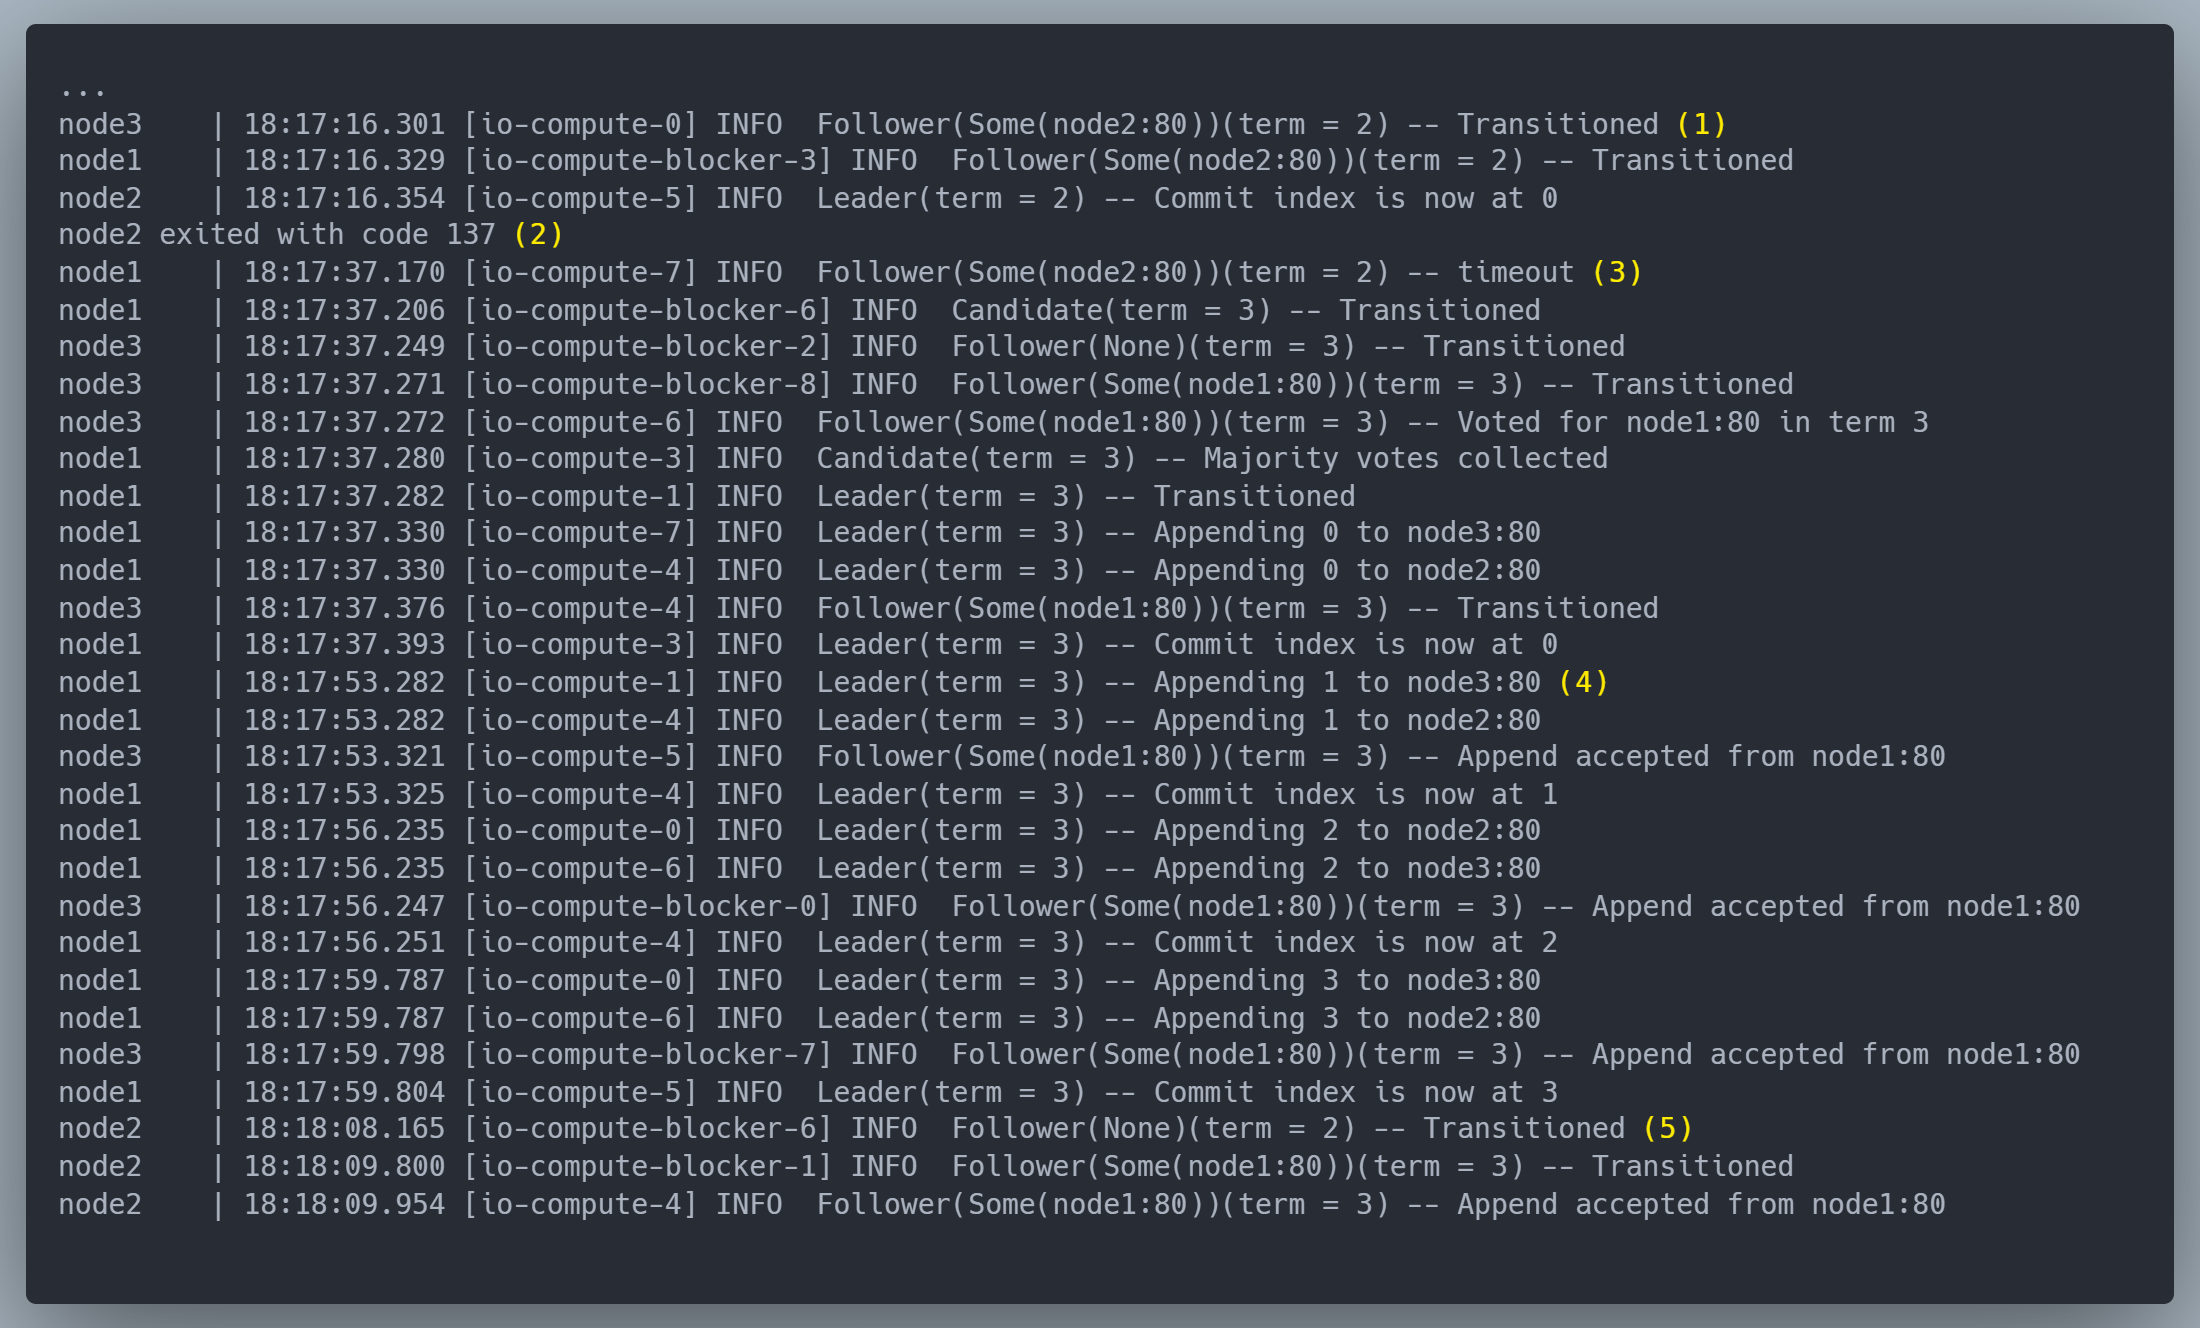
\includegraphics[width=500pt]{images/scenario_9_cluster.png}
\caption{Cluster output for the ninth scenario.}
\label{fig:scenario-9-cluster}
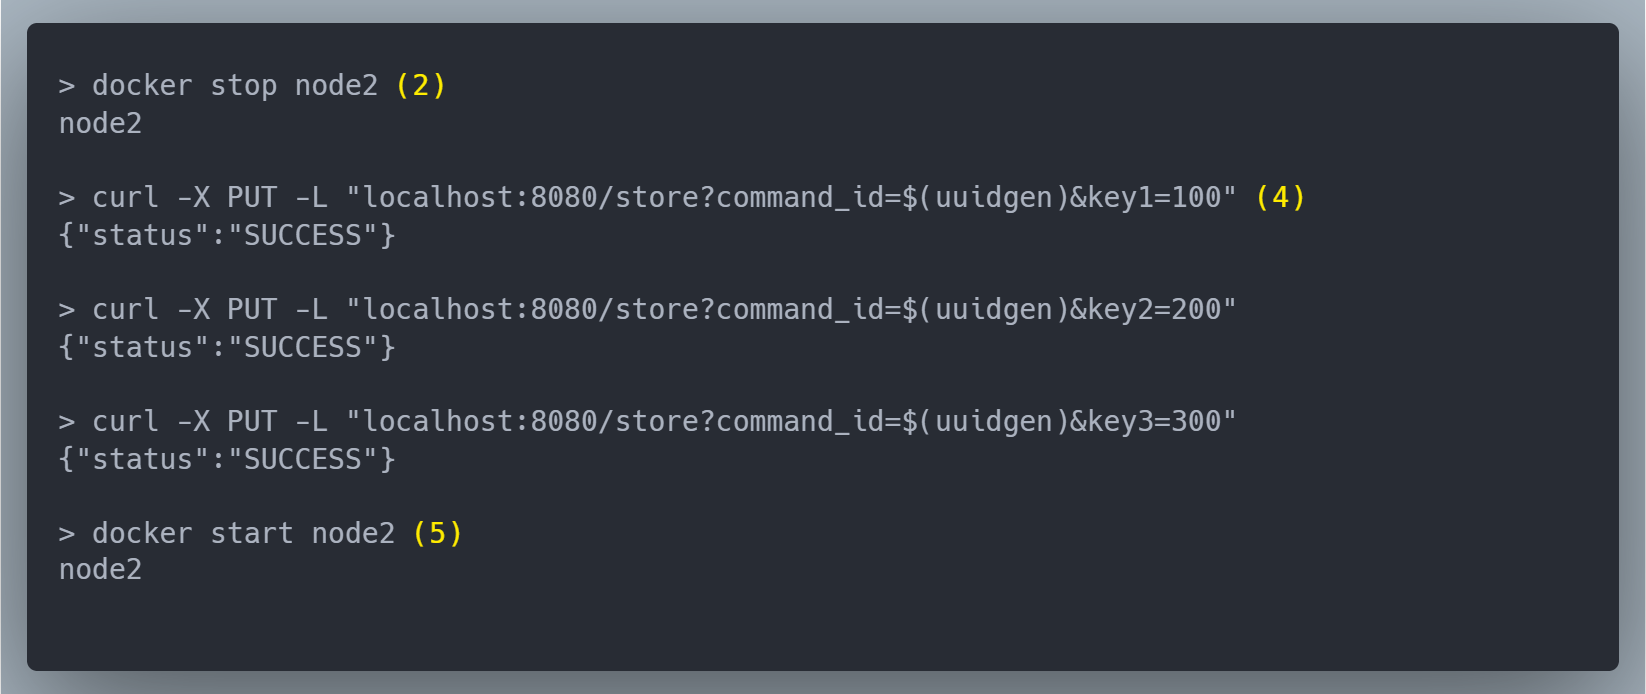
\includegraphics[width=500pt]{images/scenario_9_commands.png}
\caption{Input commands for the ninth scenario.}
\label{fig:scenario-9-commands}
\end{figure}

\begin{figure}[!ht]
\centering
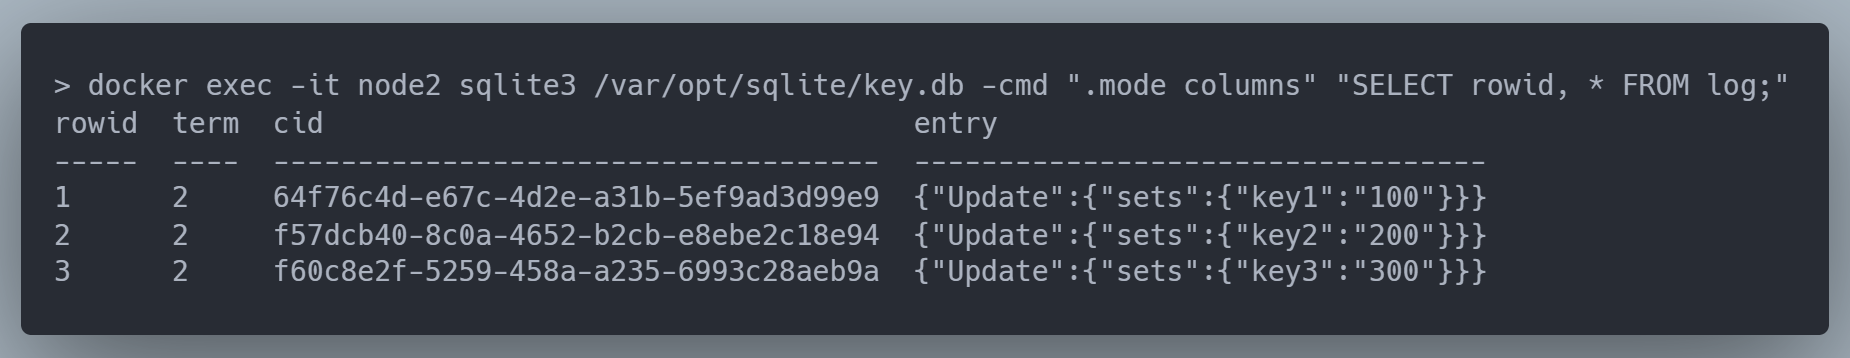
\includegraphics[width=500pt]{images/scenario_9_sqlite.png}
\caption{Input commands for the ninth scenario.}
\label{fig:scenario-9-sqlite}
\end{figure}

\subsubsection{Result}
In Figures \ref{fig:scenario-9-cluster} and \ref{fig:scenario-9-commands}, the following events are marked:
\begin{enumerate}
    \item The cluster is stable before any command is issued, with Server 2 being the leader and Servers 1 and 3 being followers.
    \item Server 2 is stopped via an external command.
    \item The leader election process begins for the next term with Server 1 ending up as the leader.
    \item Three inserts are issued via external commands and are successfully replicated throughout the cluster.
    \item Server 2 is restarted, learns the new term, and receives the log entries it missed. The internal log of Server 2 is now completely up-to-date.
\end{enumerate}

The resulting state of Server 2 can be further demonstrated by examining its local log. This is shown in Figure \ref{fig:scenario-9-sqlite}, where a \lstinline|SELECT| statement is performed against the server's Sqlite log table, using the \lstinline|sqlite3| CLI tool. The output shows the three commands in their internal representation, with all of them having the correct term and index, proving that they were correctly replicated to Server 2 after its recovery.

\subsubsection{Commentary}

These results show that Raft can indeed catch up servers that did not participate in the replication process for a while. Note that, in this scenario, the leader was chosen to be stopped. Had a follower been picked instead, the results would have been almost identical, with one key difference; no leader election process would have been necessary upon the follower's stoppage. 

\subsection{Network Partition Recovery}

This scenario simulates a network partition and demonstrates the store's recovery.

\subsubsection{Initial State}

The replicated log is empty and the cluster is stable with Server 2 as the leader, as shown under Marker 1 in Figure \ref{fig:scenario-10-cluster}.

\subsubsection{Input}

As shown in Figure \ref{fig:scenario-10-commands}, a network partition is simulated by issuing the \lstinline|docker network disconnect| command via the terminal. The partition splits the cluster into two groups; Server 1 and Server 3 are in one group, while Server 2 is in another. The partition is later resolved by using the \lstinline|docker network connect| command.

\begin{figure}[!ht]
\centering
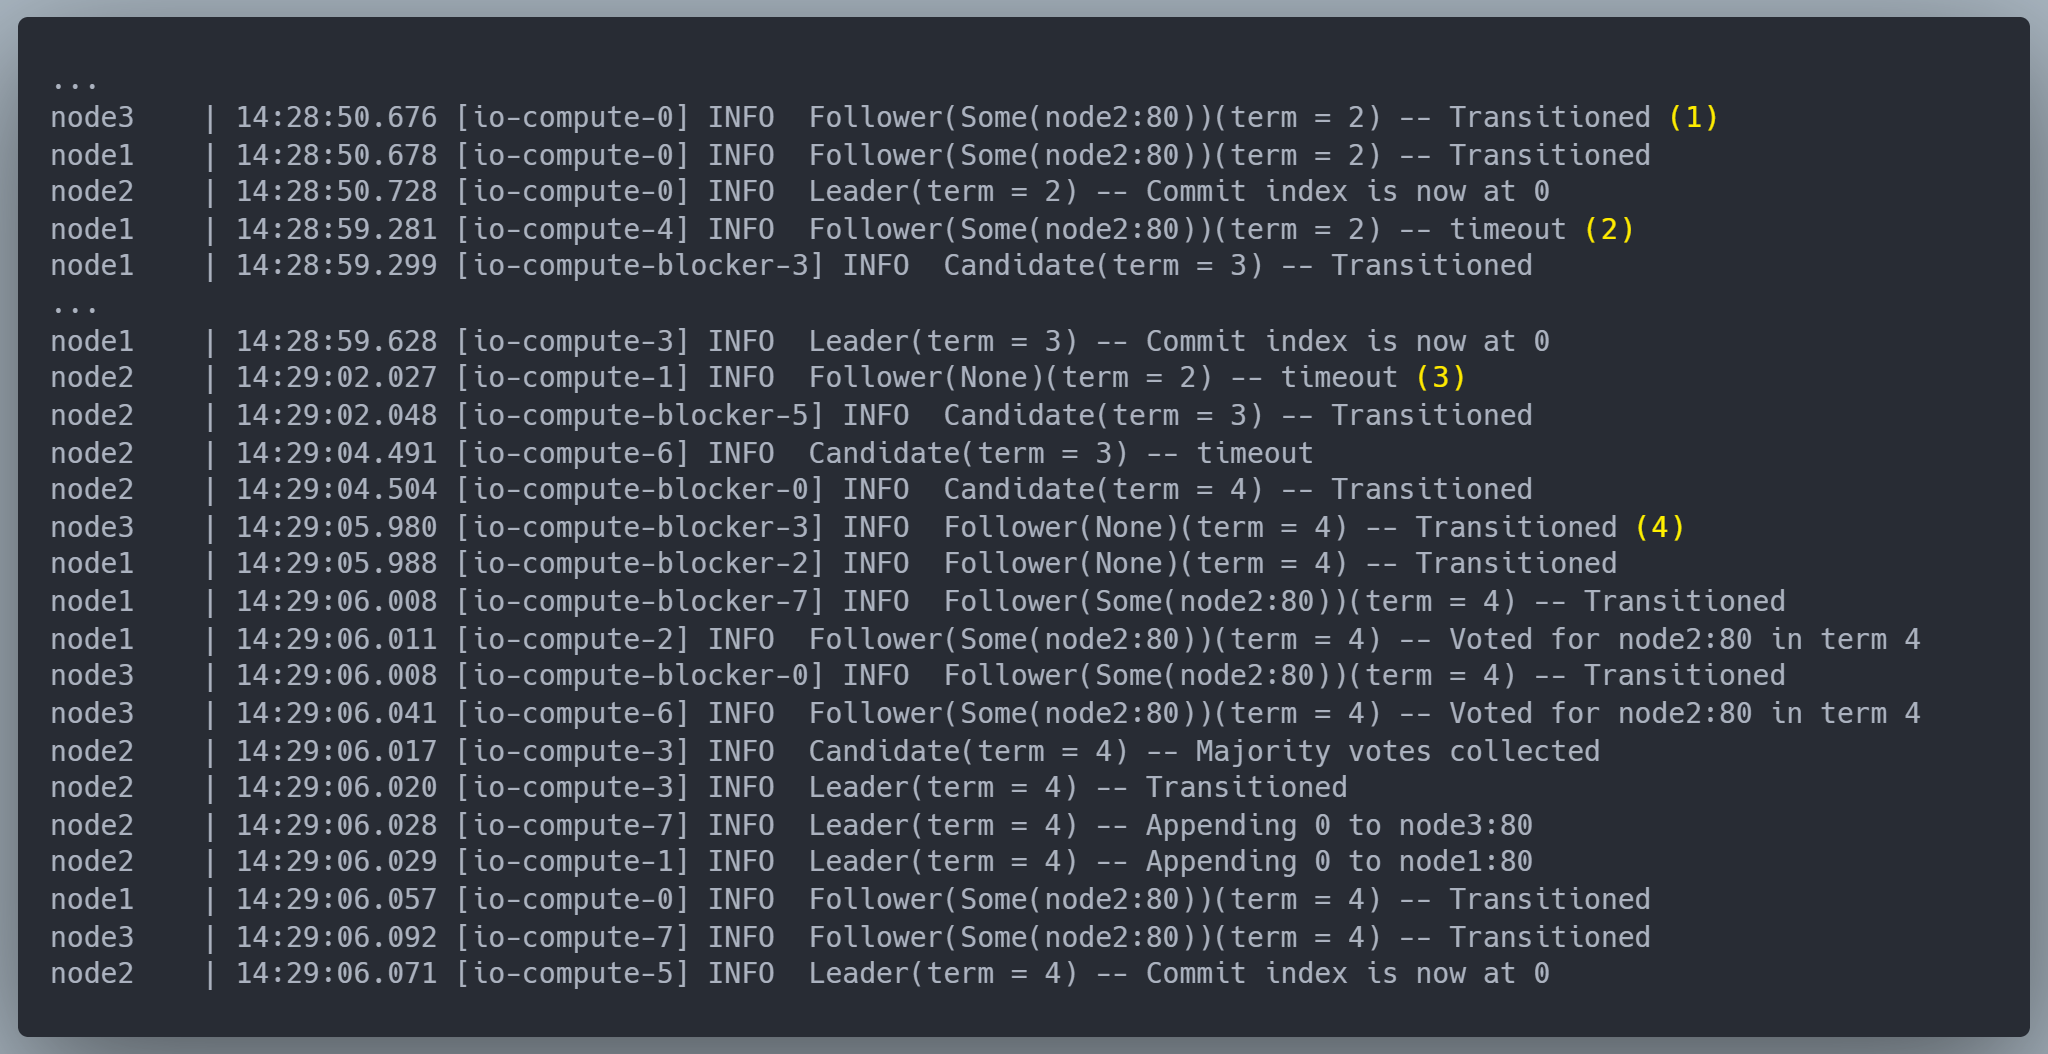
\includegraphics[width=500pt]{images/scenario_10_cluster.png}
\caption{Cluster output for the tenth scenario.}
\label{fig:scenario-10-cluster}
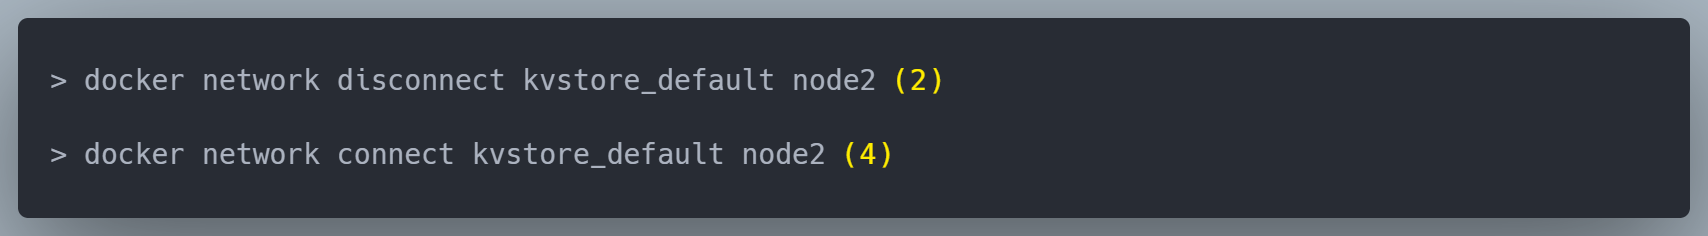
\includegraphics[width=500pt]{images/scenario_10_commands.png}
\caption{Input commands for the tenth scenario.}
\label{fig:scenario-10-commands}
\end{figure}

\subsubsection{Result}
In Figures \ref{fig:scenario-10-cluster} and \ref{fig:scenario-10-commands}, the following events are marked:
\begin{enumerate}
    \item The cluster is stable before any command is issued, with Server 2 being the leader and Servers 1 and 3 being followers.
    \item A network partition is simulated that isolates the leader from its followers. Server 1 detects that there is no viable leader, becomes a candidate for the next term, and wins the election.
    \item Server 2 detects a partition and becomes a follower, since it is unable to reach the other servers. Then, after an election timeout, it becomes a candidate for the next term and attempts to gather votes. Server 2 goes through multiple iterations of unsuccessful election attempts as it remains partitioned.
    \item The partition is resolved and Server 2 can once again reach the other servers. Server 2 then attempts to become the leader again and succeeds. During the election, the other servers adopt the term that Server 2 had reached while partitioned, since its larger than their own terms. 
\end{enumerate}

\subsection{Leader Reelection with Populated Log}

This scenario shows the store's fault tolerance with a populated log.

\subsubsection{Initial State}
The replicated log is empty and the cluster is stable with Server 1 as the leader, as shown under Marker 1 in Figure \ref{fig:scenario-11-cluster}.

\subsubsection{Input}
As shown in Figure \ref{fig:scenario-11-commands}, the log is initially populated by running the \lstinline{concurrent_read_writes} script. This ensures that the log is fairly long and complex. Then, the leader is stopped by issuing a \lstinline{docker stop} command. Finally, the values of the 10 keys created by the \lstinline{concurrent_read_writes} script are requested, using \lstinline{curl}.

\begin{figure}[!ht]
\centering
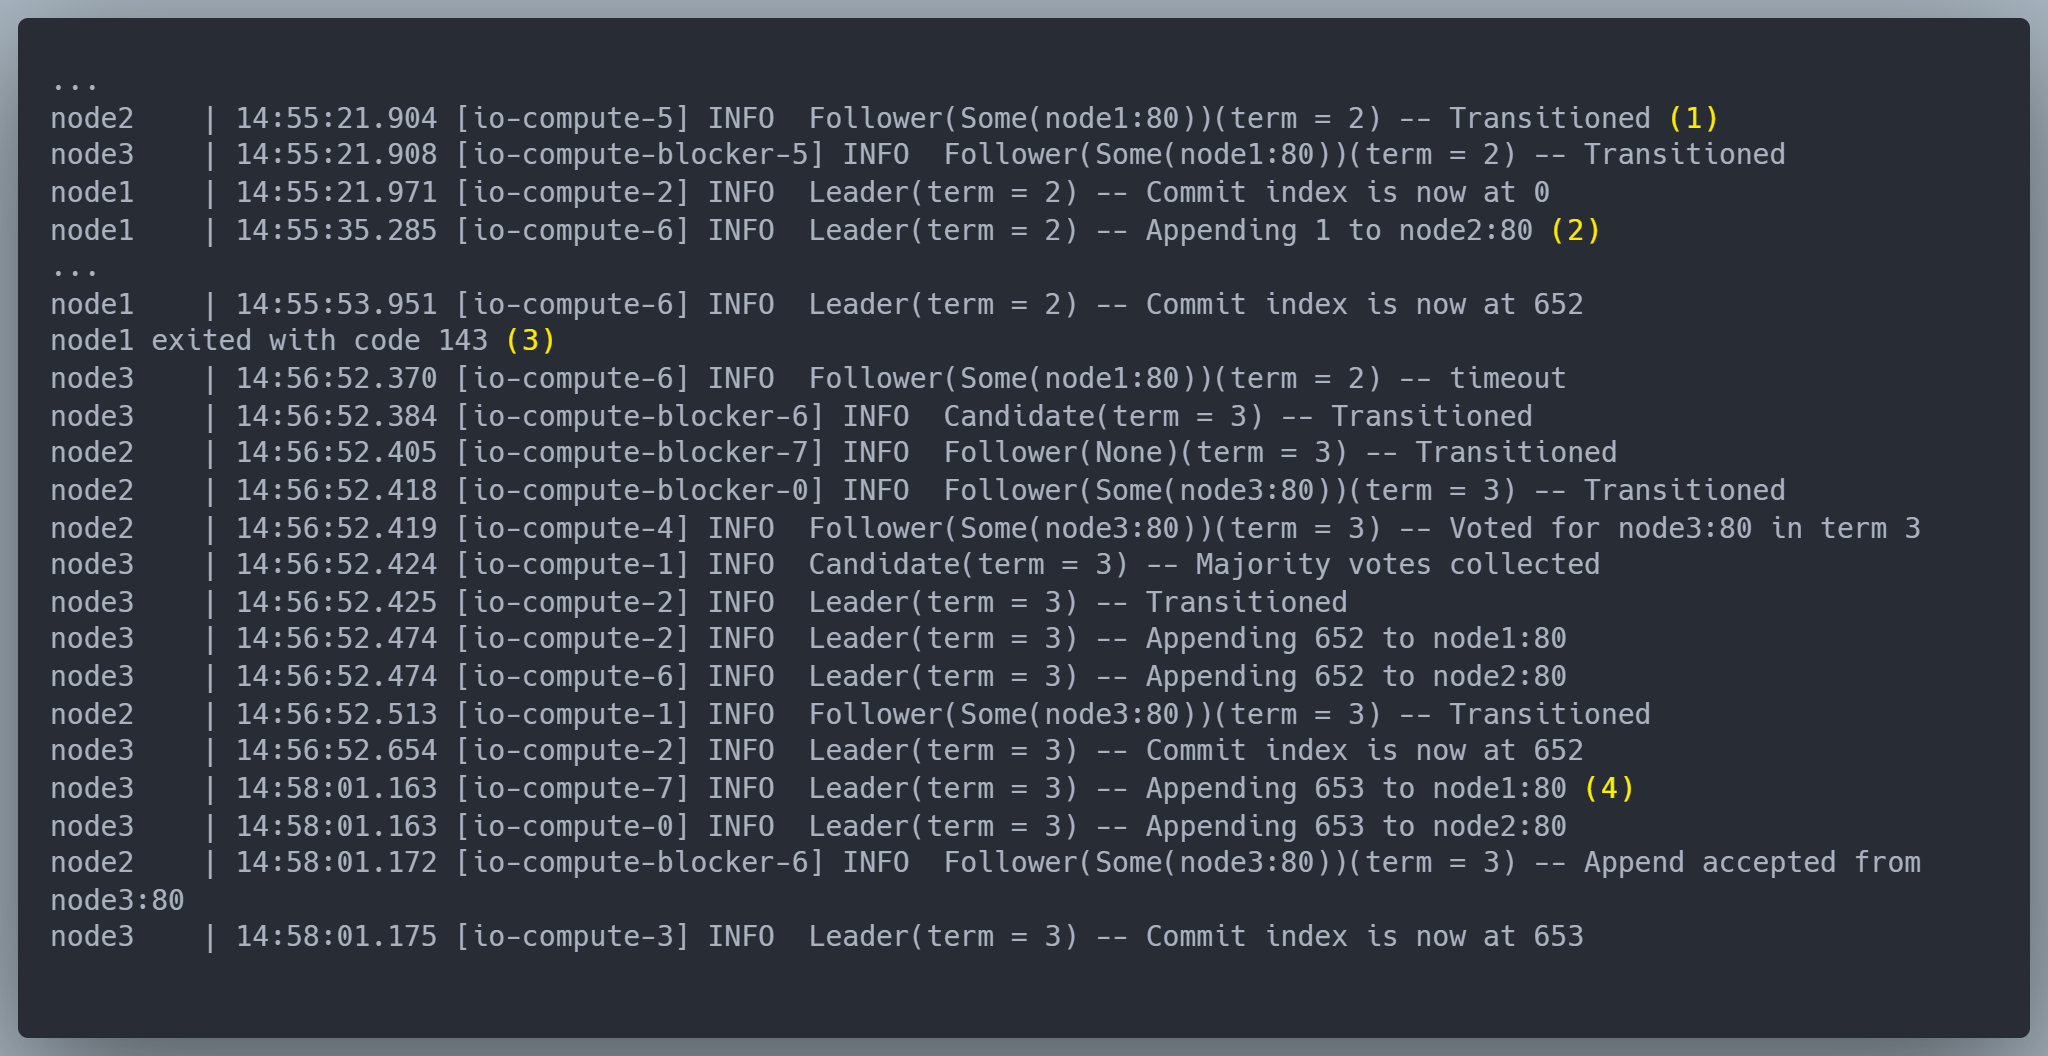
\includegraphics[width=500pt]{images/scenario_11_cluster.png}
\caption{Cluster output for the eleventh scenario.}
\label{fig:scenario-11-cluster}
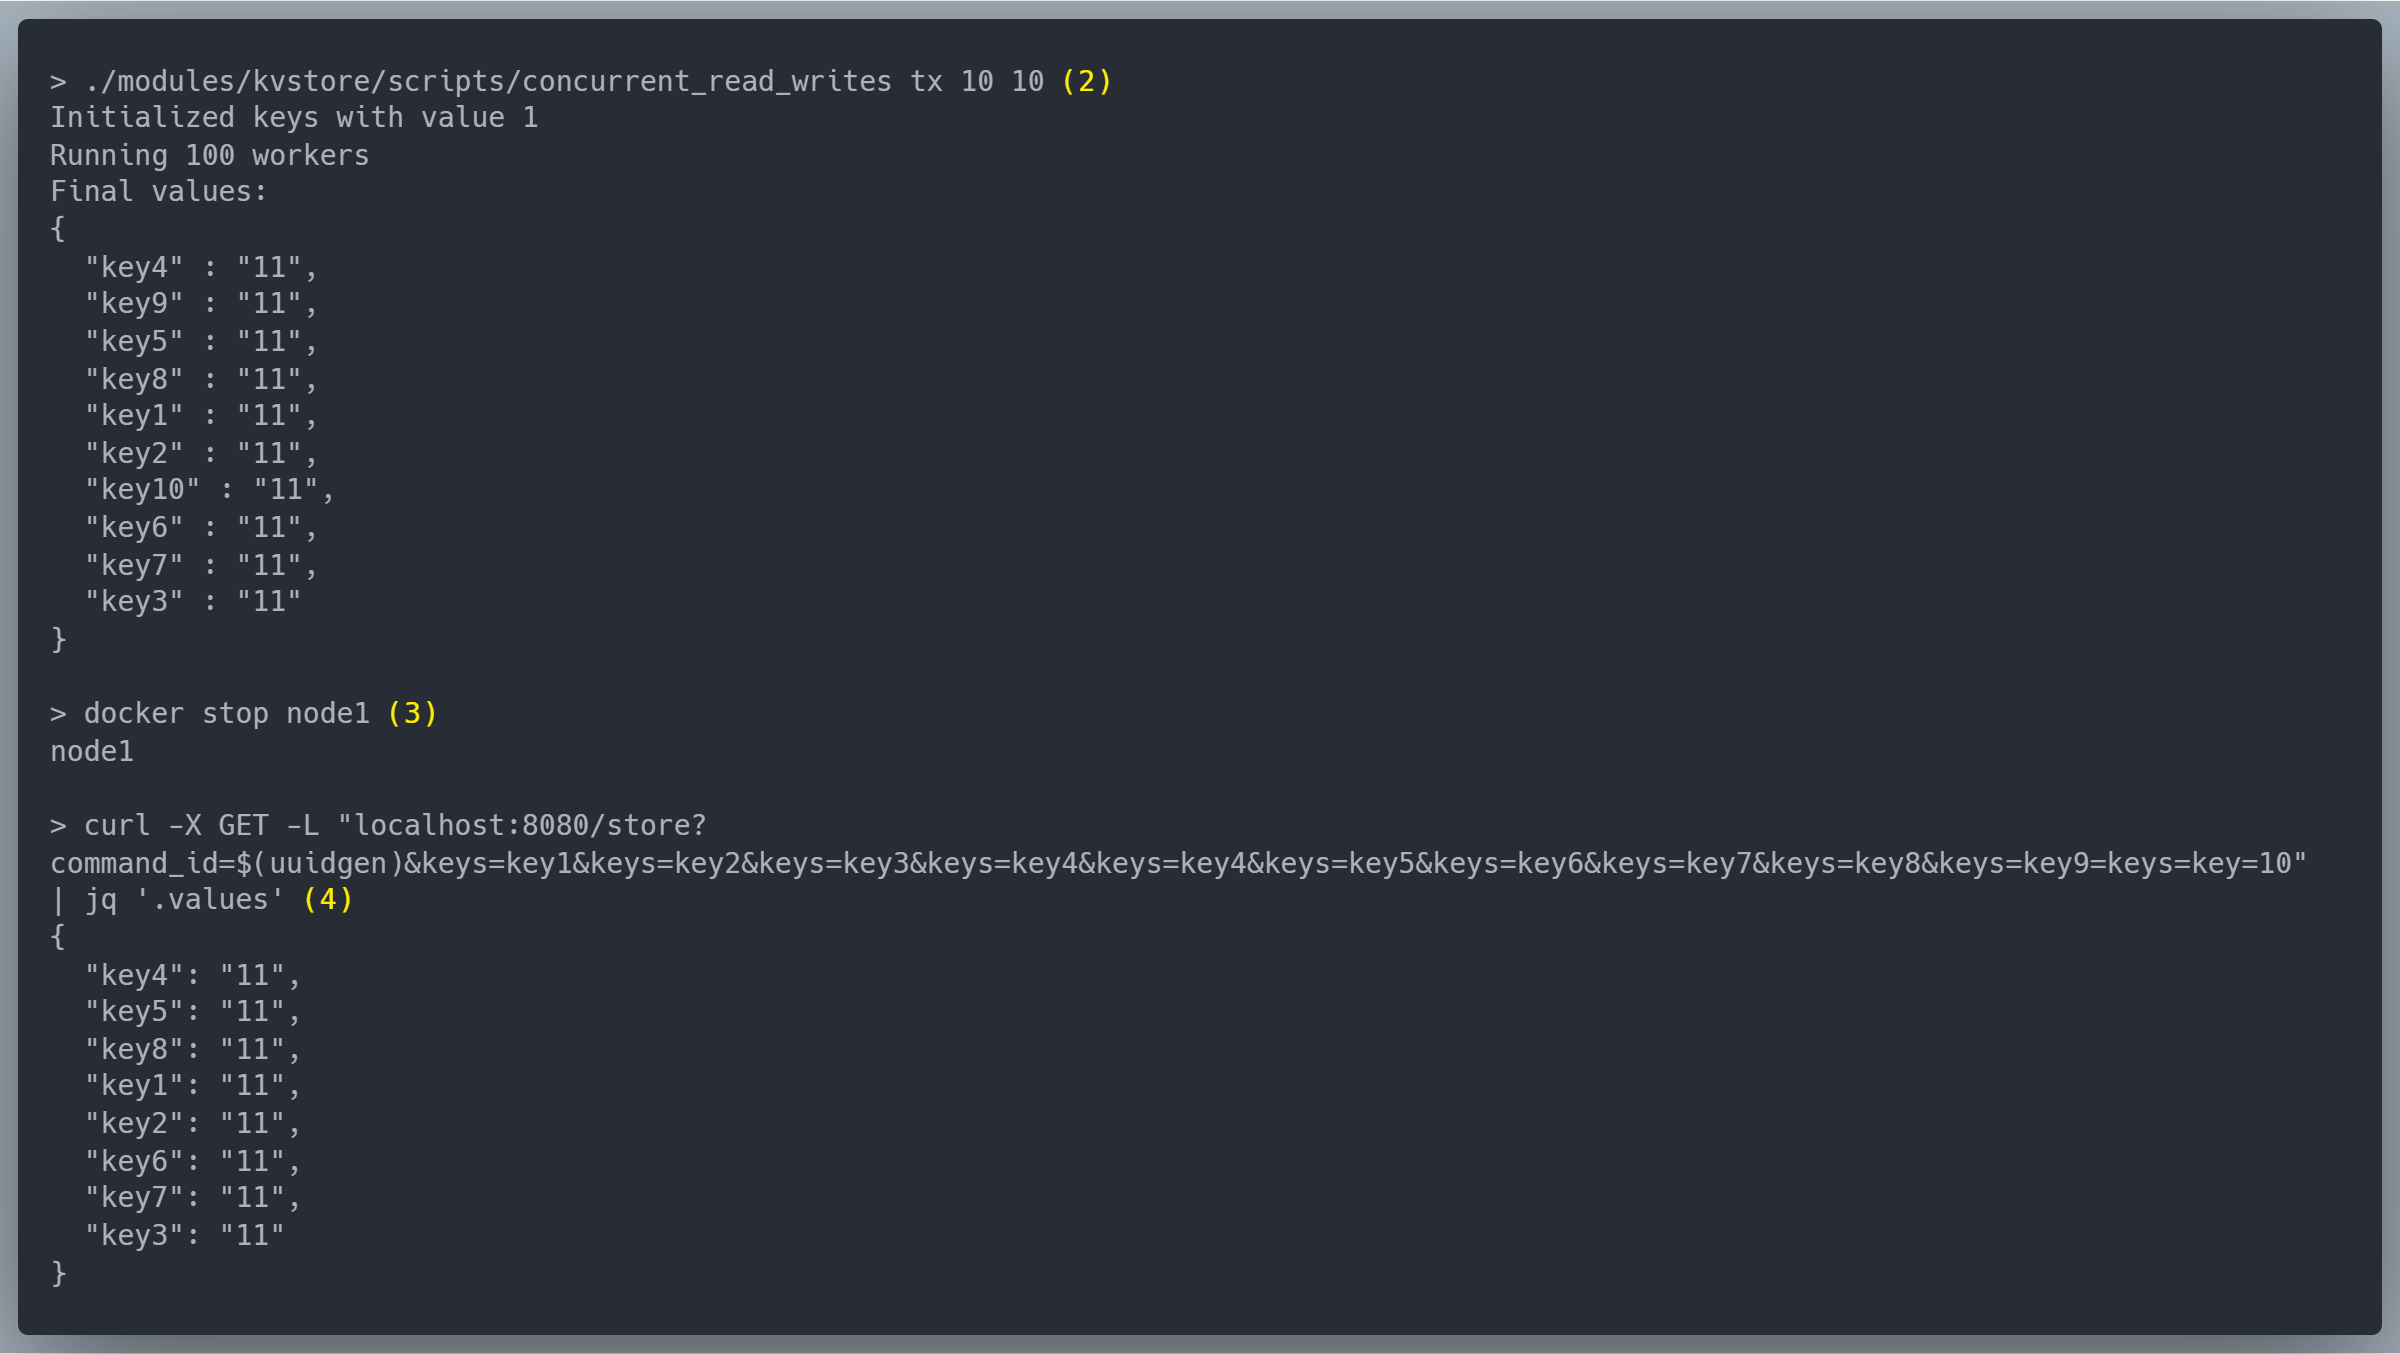
\includegraphics[width=500pt]{images/scenario_11_commands.png}
\caption{Input commands for the eleventh scenario.}
\label{fig:scenario-11-commands}
\end{figure}

\subsubsection{Result}
In Figures \ref{fig:scenario-11-cluster} and \ref{fig:scenario-11-commands}, the following events are marked:
\begin{enumerate}
    \item The cluster is stable before any command is issued, with Server 1 being the leader and Servers 2 and 3 being followers.
    \item The \lstinline{concurrent_read_writes} script is run and the commit index reaches 652.
    \item A crash is simulated in Server 1, which triggers an election, with Server 3 ending up as the new leader.
    \item The values of the keys that were previously inserted are requested. The new leader responds, returning the correct values.
\end{enumerate}

\subsubsection{Commentary}

These results clearly show that the state machine is correctly replicated, enabling the cluster to continue to progress in case of leader failures. Also note that the same would have been true had the leader been partitioned instead of crashing.

\subsection{Command Rejection when Non-Linearizable}

This scenario shows how the store enforces linearizability in the face of duplicate commands. Linearizability is explained in Section \ref{linearizable-semantics}.

\subsubsection{Initial State}
The replicated log is empty and the cluster is stable with Server 3 as the leader, as shown under Marker 1 in Figure \ref{fig:scenario-12-cluster}.

\subsubsection{Input}
Two identical \lstinline|PUT| requests are sent via the terminal with \lstinline|curl|, using the same command id. In addition to the \lstinline|-L| flag that was described in Scenario \ref{L-flag}, the HTTP response codes are shown using the \lstinline|-I| flag. 

\begin{figure}[!ht]
\centering
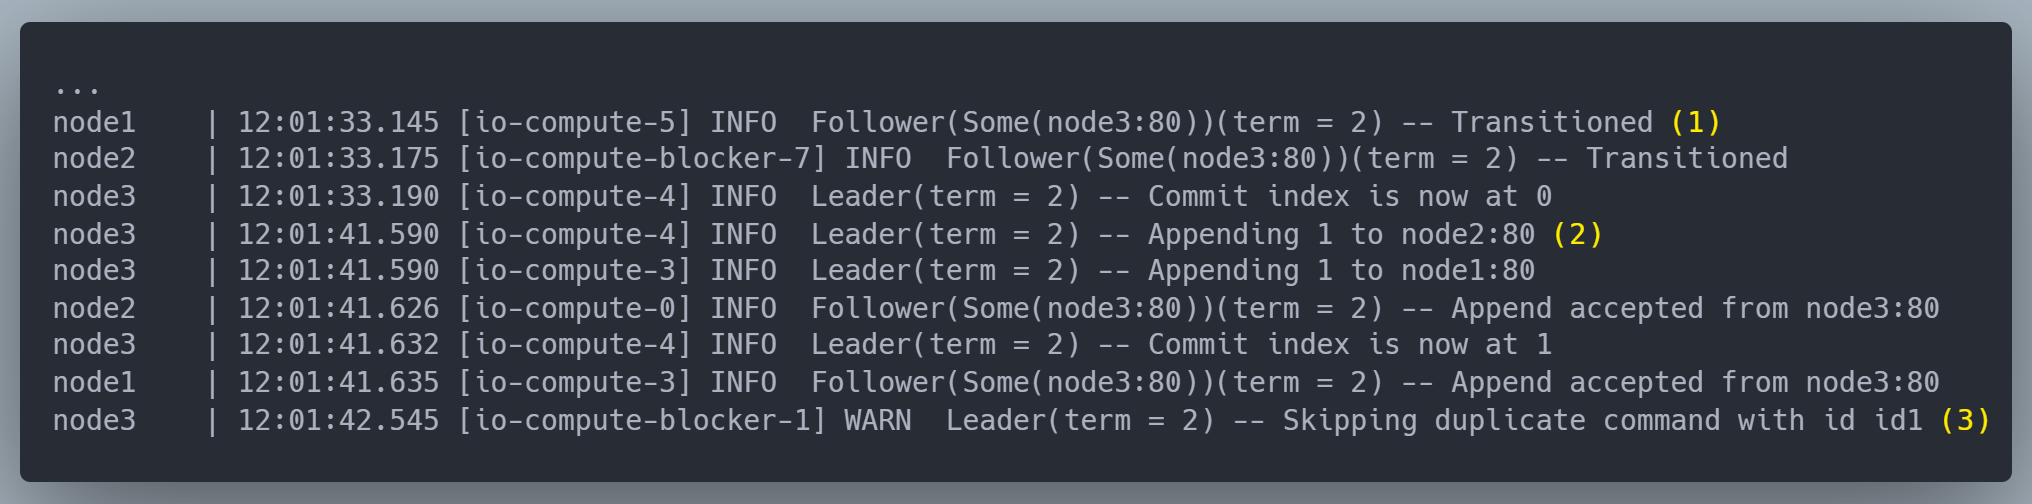
\includegraphics[width=500pt]{images/scenario_12_cluster.png}
\caption{Cluster output for the twelfth scenario.}
\label{fig:scenario-12-cluster}
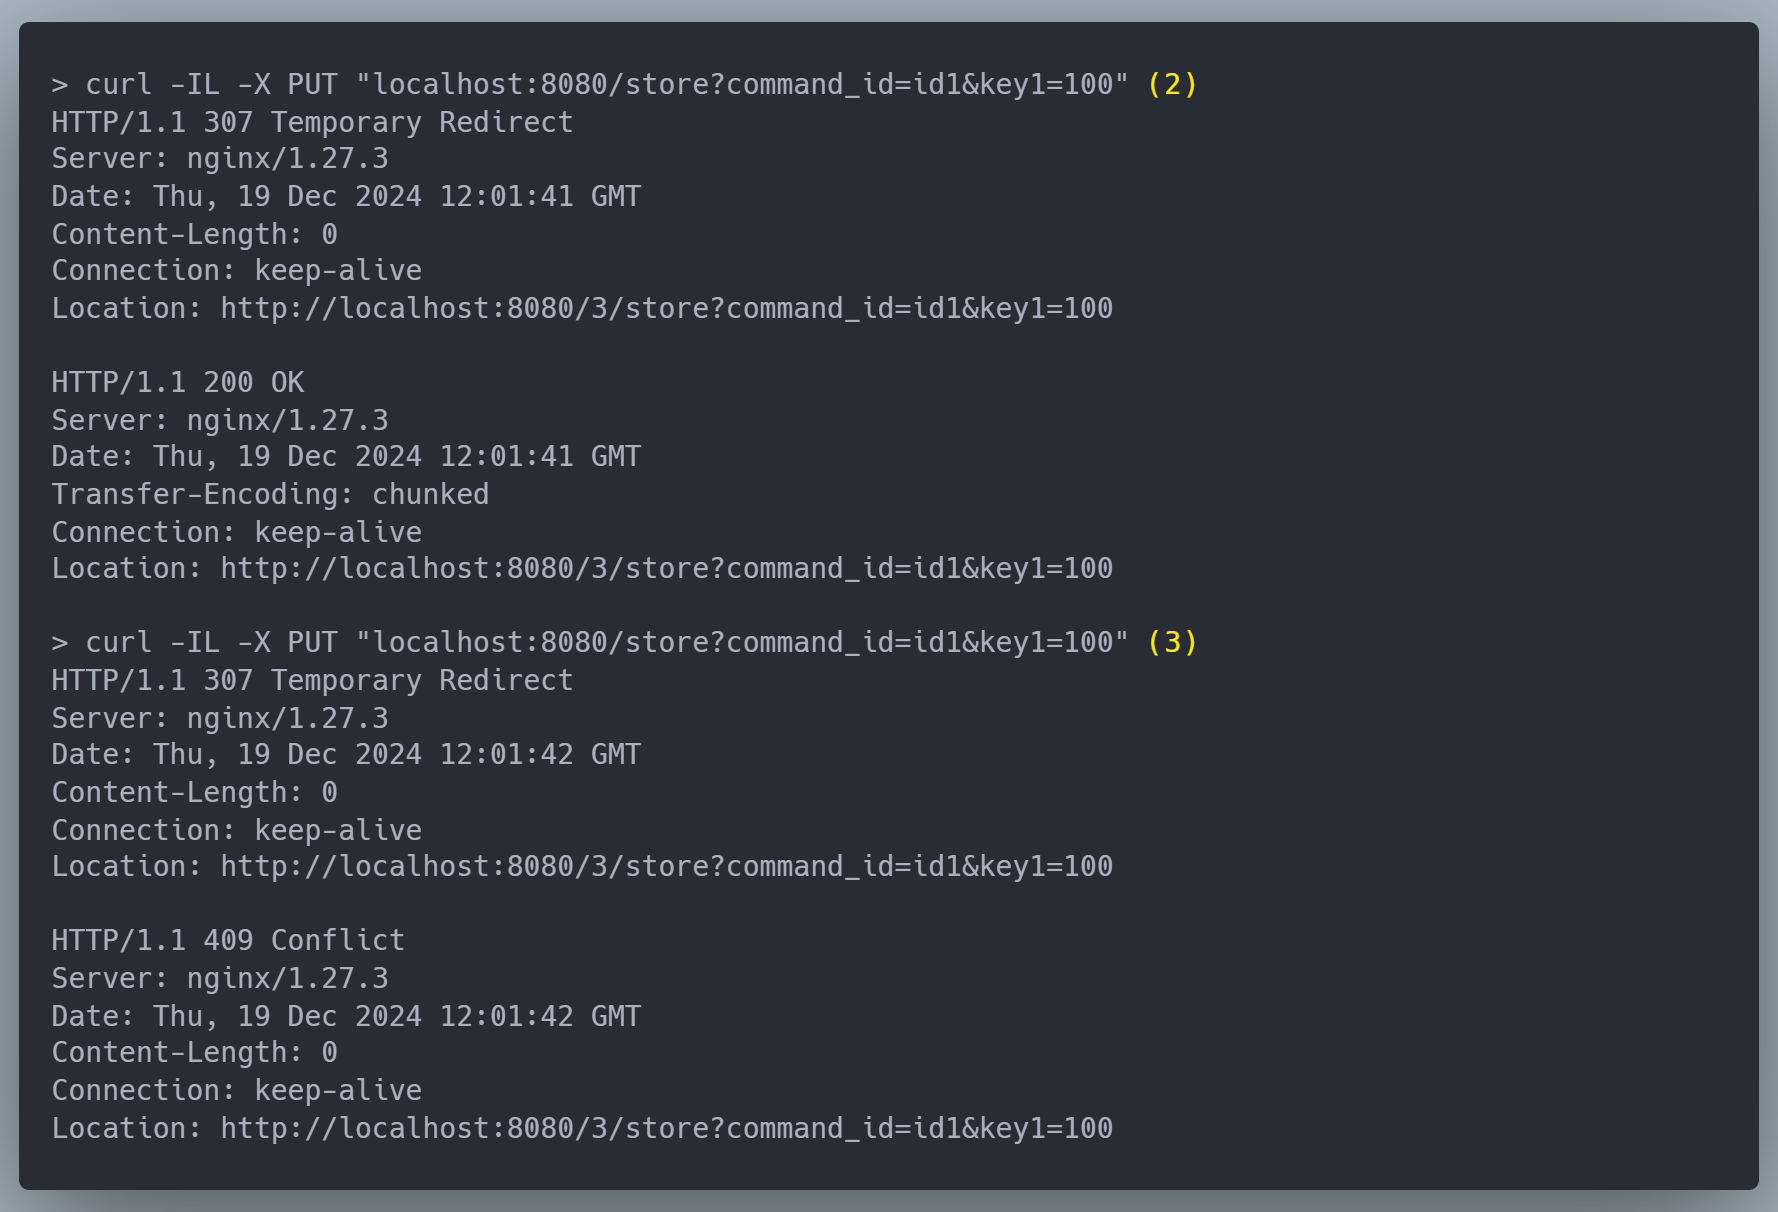
\includegraphics[width=500pt]{images/scenario_12_commands.png}
\caption{Input commands for the twelfth scenario.}
\label{fig:scenario-12-commands}
\end{figure}

\subsubsection{Result}
In Figures \ref{fig:scenario-12-cluster} and \ref{fig:scenario-12-commands}, the following events are marked:
\begin{enumerate}
    \item The cluster is stable before any command is issued, with Server 3 being the leader and Servers 1 and 2 being followers.
    \item The first request is issued via the terminal. The store redirects to the leader server, which accepts the request and commits the command.
    \item The second request is issued, which is rejected after being redirected to the leader. The 409 HTTP code is returned, indicating that the request conflicts with the server's state \cite{409-status-code}.
\end{enumerate}
